% Anonymous ICML-style research manuscript. Compile from the /work directory.
% Official template files are used without modification.
\documentclass{article}
\usepackage{microtype}
\usepackage{graphicx}
\usepackage{booktabs}
\usepackage{hyperref}
\newcommand{\theHalgorithm}{\arabic{algorithm}}
\usepackage[preprint]{template/icml2026}
\usepackage{amsmath,amssymb,mathtools,amsthm}
\theoremstyle{plain}
\newtheorem{proposition}{Proposition}
\newtheorem{corollary}{Corollary}
\newtheorem{theorem}{Theorem}
\newcommand{\simp}{\Delta^{K-1}}
\newcommand{\E}{\mathbb{E}}
\newcommand{\Prob}{\mathbb{P}}
\newcommand{\ind}{\mathbf{1}}
\newcommand{\R}{\mathcal{R}}
\newcommand{\Udel}{U_{\Delta}}
\newcommand{\UF}{U_{F}}
\newcommand{\norm}[1]{\left\lVert #1\right\rVert}
\icmltitlerunning{A Face-Aware Audit of Conformal Regions for Compositions}

\begin{document}
\twocolumn[
\icmltitle{When Simplex Volume Is Not Enough:\\
A Face-Aware Audit of Conformal Regions for Compositions}
\begin{icmlauthorlist}
\icmlauthor{Anonymous Authors}{anon}
\end{icmlauthorlist}
\icmlaffiliation{anon}{Anonymous affiliation}
\icmlkeywords{conformal prediction, compositional responses, structural zeros, reliability evaluation}
\vskip 0.3in
]
\printAffiliationsAndNotice{}

\begin{abstract}
Conformal regions for compositional responses can satisfy marginal coverage while excluding important response strata, and intrinsic full-simplex volume cannot detect changes confined to a face. We assemble a face-aware evaluation protocol that separates observed-composition coverage, observable-group and realized-boundary diagnostics, and explicitly chosen reference masses; the contribution is an evaluation synthesis and an independently implemented benchmark, not a new conformal algorithm or validity theorem. A closed-set control has identical ambient volume before and after adding a supported face, yet its response coverage increases by exactly $0.35$ in our mixture law. Across 50 seeds, three dimensions, and two synthetic laws, pooled L2 attains source-mixture marginal coverage $0.90065$ but difficult-group coverage $0.56421$; smoothed CLR ($\varepsilon=10^{-6}$) regions in the source mixture combine estimated ambient mass $0.999845$ with boundary-response coverage $0.71532$. Scaling and group calibration improve observable-group reliability but reduce source boundary coverage, while oracle weighting and group calibration recover shifted marginal coverage only under their specified assumptions. Ten frozen contrasts with approximate multiplicity-adjusted bootstrap intervals, complete dimension-resolved results, and explicit Monte Carlo limitations support a bounded audit interpretation rather than a universal ranking.
\end{abstract}

\section{Introduction}
\label{sec:intro}
A composition is a nonnegative vector whose entries sum to one. Such a response may describe proportions, but sharing a simplex domain with class probabilities does not make it an unknown probability parameter. This paper predicts the next \emph{observed composition}, including exact zeros. It does not infer a class label, a latent clean vector, or a true conditional class-probability vector. Standard conformal calibration can cover this observed response without choosing a special simplex-specific validity argument \citep{angelopoulos2021gentle}; evaluating the resulting region still requires deciding which reliability events and which notion of size matter.

Two separations motivate our audit. First, marginal coverage averages errors across covariates and response strata. A difficult observable group can be poorly covered even when the overall rate is near nominal. Second, intrinsic $(K-1)$-dimensional volume assigns zero mass to every proper face of the $K$-part simplex. Consequently, equal ambient volumes need not imply equal coverage when responses have structural zeros. Neither a small volume nor an almost full-volume region resolves this reliability question.

We make these separations explicit rather than propose a replacement conformal method. Our audit reports simultaneous composition coverage, coverage within a prespecified observable group, diagnostic coverage after observing zero status, and normalized masses on the full simplex and on individual faces. A frozen mixture of these geometric reference measures summarizes size, but is neither a response law nor application utility. It is also incomplete: for $K\geq3$, codimension-one probes still miss lower-dimensional face intersections, including vertices.

The empirical contribution is a controlled, independently implemented comparison of established score and calibration constructions. We complete $50\times3\times2=300$ seed/dimension/law cells with a common learned predictor and matched evaluations. The source-mixture example in Figure~\ref{fig:audit} demonstrates why the expanded report changes interpretation. Near-nominal marginal coverage coexists with different observable-group and boundary failures. Under a group-frequency shift, standard weighting and group calibration recover aggregate coverage, but their assumptions and guarantees differ. The study is deliberately limited to synthetic responses, one structural face, one learner, and one nominal level.

Our contributions are therefore scoped as follows: (i) an explicit geometric control, including closed sets, separating ambient mass from boundary-response reliability; (ii) a reproducible audit combining standard validity statements with component-wise reference masses; and (iii) complete evidence for ten frozen aggregate comparisons, including adverse error redistribution, reference dependence, dimension heterogeneity, and numerical resolution limits. We claim no new conformal theorem, algorithm, state of the art, or priority over an unrestricted literature.

\section{Related Work and Target Distinctions}
\label{sec:related}
Split conformal prediction calibrates a fixed scalar nonconformity score independently of model fitting. Scalar-regression constructions and their coverage/length/computation comparisons provide useful protocol precedents \citep{lei2016distributionfree}. The general score-set formulation and feature- or size-stratified diagnostics emphasize that marginal coverage is not input-conditional validity \citep{angelopoulos2021gentle}. We apply these established distinctions to observed simplex-valued responses and add explicit geometric reference strata.

Conformal classification covers a \emph{label}, even when softmax probabilities determine its score. Adaptive and regularized label-set methods illustrate that marginal coverage and difficulty-dependent behavior can diverge \citep{angelopoulos2020uncertaintysets}; label-set cardinality is not the size of a composition region. Conformalized credal sets instead target probability-valued responses using calibrated distribution-distance or likelihood scores \citep{javanmardi2024credal}. Their noisy-target discussion explicitly distinguishes coverage of observed annotation frequencies from coverage of latent probabilities. We retain that distinction and do not transfer latent-target guarantees to our observed-response experiment. We do not reproduce their neural or second-order predictors; this benchmark isolates score/calibration behavior under one shared learner, rather than compare complete application pipelines.

Oracle covariate-shift conformal prediction assumes an unchanged response law given covariates, overlap, and a known density ratio; its test-point atom at infinity is part of the construction \citep{tibshirani2019covariateshift}. Our weighting comparison uses exactly that privileged information. Group calibration has a separate transport argument when the complete within-group law is preserved. Neither mechanism implies nominal coverage conditional on an unobserved future structural zero. Literature access was deliberately restricted to these five read sources; this section is not an exhaustive survey or a novelty certification.

\section{Audit Method and Comparison Protocol}
\label{sec:method}
\subsection{Prediction target and calibration}
Let $\simp=\{y\in\mathbb{R}^K:y_j\geq0,\sum_jy_j=1\}$ and $F_j=\{y\in\simp:y_j=0\}$. Training produces a fixed predictor $f_T(x)\in\simp$ and, when needed, positive train-only scales. For a measurable finite scalar score $s_T$, use $m$ independent calibration observations and
\begin{equation}
 \begin{aligned}
 k&=\lceil(m+1)(1-\alpha)\rceil,\\
 \R(x)&=\{y\in\simp:s_T(x,y)\leq q\},
 \end{aligned}
 \label{eq:split}
\end{equation}
where $q$ is the $k$th calibration score, or $+\infty$ if $k>m$. Membership uses the original response and a weak inequality, not a transformed-response surrogate or interpolated percentile. Here $m=499$, $\alpha=0.1$, and $k=450$.

We compare ten nonoracle constructions: TV (half L1), L2, jointly calibrated Linf, Hellinger, positive-epsilon centered log-ratio (CLR) scores at $10^{-6}$ and $10^{-2}$, unadjusted coordinate intervals, Bonferroni coordinate intervals, training-scale L2, and observable-group Mondrian L2. TV/L1 is one geometry in different units, not two baselines. The unadjusted coordinate intersection is an intentional joint-coverage negative control. Scaled L2 pools scores $\norm{y-f_T(x)}_2/\sigma_G$; Mondrian L2 instead calibrates separate corrected ranks within the observed binary group $G$. An eleventh, oracle-weighted L2 comparator is evaluated under shift. All formulas, floors, ranks, and weight conventions appear in Appendix~\ref{app:methods}.

\subsection{Reliability and reference mass}
We measure simultaneous composition coverage $C=\Prob\{Y\in\R(X)\}$, observable-group rates $C_{G=g}$, and mixture-law rates $C_{B=b}$, where $B=1$ denotes the realized event $Y_K=0$. The latter is a post-outcome diagnostic, never a test-time calibration input. No boundary rate is defined for the interior-only law.

Let $\Udel$ be uniform intrinsic volume on $\simp$ and $U_{F_j}$ uniform intrinsic volume on $F_j$. The frozen reference is
\begin{equation}
 Q=\tfrac12\Udel+\tfrac1{2K}\sum_{j=1}^K U_{F_j}.
 \label{eq:Q}
\end{equation}
For a fitted region, define $V=\E_X\Udel(\R(X))$, $A_j=\E_XU_{F_j}(\R(X))$, and
\begin{equation}
 E_Q=\tfrac12 V+\tfrac1{2K}\sum_j A_j.
 \label{eq:mass}
\end{equation}
These normalized masses, unlike raw volumes in different dimensions or score radii in different units, have an explicit common reference interpretation. We always retain the supported-face component $A_K$: averaging faces dilutes its contribution by $1/K$. Smaller mass describes size only; it is not superiority when reliability differs. $Q$ is not the response distribution, is not utility, and is not invariant to replacing the reference weights.

The audit evaluates the \emph{same} fitted regions with and without the expanded diagnostics; this is a reporting ablation, not retraining. Other frozen comparisons isolate support change, scaling versus group calibration, oracle weighting under shift, coordinate multiplicity correction, two CLR smoothings, and TV/L1 equivalence. Sensitivity replaces the ambient weight by $\rho\in\{0.25,0.5,0.75\}$ using already measured components, without choosing a favorable weight.

\section{Mathematical Scope of the Audit}
\label{sec:theory}
The following statements organize standard validity facts and elementary geometry; none is offered as a new conformal theorem. Full proofs and boundary cases are in Appendix~\ref{app:proofs}.

\begin{proposition}[Fixed-score split validity]
\label{prop:split}
Conditional on independent training $T$, let $0<\alpha<1$ and suppose the $m$ calibration pairs and a new pair are exchangeable. Then \eqref{eq:split} has coverage at least $k/(m+1)\geq1-\alpha$, allowing ties. If all scores are almost surely pairwise distinct, coverage equals $k/(m+1)$; conditional i.i.d. atomless scores suffice for this additional assumption.
\end{proposition}
A continuous score formula alone does not ensure no ties. Training-only scaling and any fixed positive-epsilon CLR are simply score choices under this result. They supply no automatic nominal group, boundary, latent-target, or fixed-input guarantee. Bonferroni coordinate calibration at $\alpha/K$ gives joint marginal coverage by a union bound; separate coordinate calibration at $\alpha$ does not.

\begin{proposition}[Closed-set ambient blind spot]
\label{prop:geometry}
For $K\geq3$, let $A=\{y\in\simp:y_K\geq1/2\}$ and $A^+=A\cup F_K$. Both are closed, and
\begin{equation}
 \begin{gathered}
 \Udel(A)=\Udel(A^+)=2^{-(K-1)},\\
 U_{F_K}(A)=0,\qquad U_{F_K}(A^+)=1,\\
 Q(A^+)-Q(A)=1/(2K).
 \end{gathered}
 \label{eq:control}
\end{equation}
If the response has probability $0.35$ in the relative interior of $F_K$ and otherwise lies in the simplex interior, then $\Prob(Y\in A^+)-\Prob(Y\in A)=0.35$.
\end{proposition}
These are exact constants for constructed controls, not measurements of fitted norm-score regions. The result follows because a face is ambient-null; on every other face, its intersection with $F_K$ is also null. Conversely, even $Q$ is blind to lower-dimensional intersections. A closed set and its union with an excluded vertex can have identical $Q$ but different coverage under a vertex atom.

\begin{proposition}[Conditional scope and group transport]
\label{prop:group}
Marginal coverage $1-\alpha$ implies only $C_H\geq\max\{0,1-\alpha/p\}$ for an event $H$ of probability $p>0$. Group-Mondrian calibration gives coverage at least $1-\alpha$ within each prespecified prediction-time observable group under i.i.d. source sampling. This transports to target groups if their full within-group joint laws of $(X,Y)$ are unchanged and target groups have source support.
\end{proposition}
For difficult-group prevalence $0.2$, marginal $0.9$ permits group coverage $0.5$. For boundary prevalence $0.35$, the generic bound is only $5/7$, not $0.9$. Preserving $Y\mid X$ alone is insufficient for the group-transport statement if $X\mid G$ changes. Oracle weighting instead gives target \emph{marginal} validity under its density-ratio and invariant-$Y\mid X$ assumptions \citep{tibshirani2019covariateshift}. All guarantees average over calibration and new-test randomness; none promises the nominal rate in every realized seed.

\begin{figure*}[t]
\centering
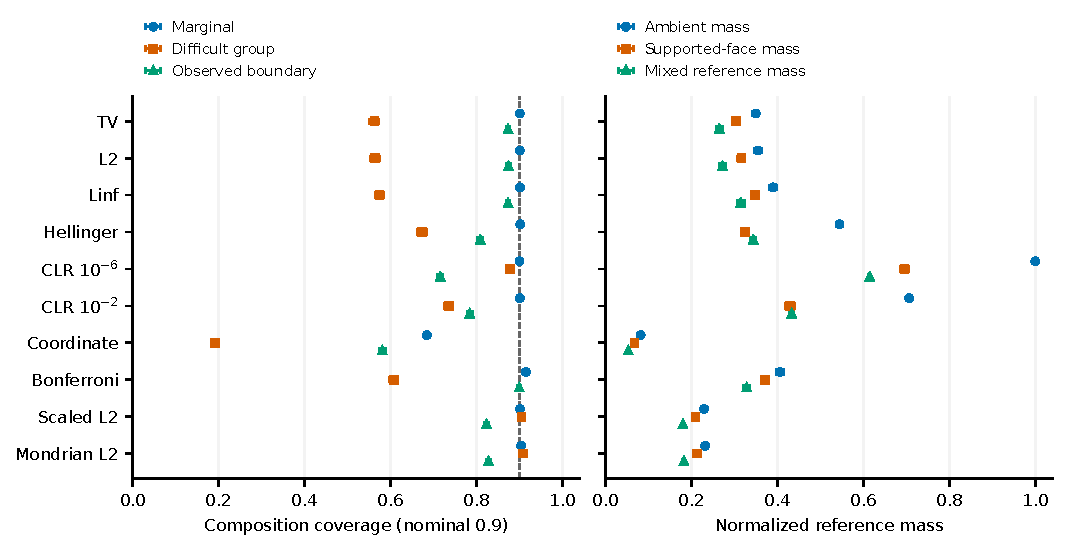
\includegraphics[width=\textwidth]{figures/audit.pdf}
\caption{Complete ten-method source-mixture audit, equally averaging $K=3,5,10$ within each of 50 seeds. Left: observed-composition coverage overall, in the difficult observable group, and among realized boundary responses; dashed line is $0.9$. Right: normalized ambient, supported-face, and frozen mixed reference masses, not response probabilities. Bars are pointwise descriptive 95\% seed-bootstrap intervals. CLR $10^{-6}$ has near-saturated, \emph{not exactly unit}, estimated ambient mass. Source: \texttt{artifacts/analysis/summary\_by\_law.csv}.}
\label{fig:audit}
\end{figure*}

\section{Experiments}
\label{sec:experiments}
\subsection{Frozen design, stages, and quality controls}
The two synthetic laws use $K\in\{3,5,10\}$ and independent splits of 1,500 training, 499 calibration, and 2,000 test observations \emph{per regime}. Inputs are $X=(U_1,U_2,G)$, with independent uniform $U_i\in[-1,1]$. A smooth softmax determines interior Dirichlet means; concentration is 80 for $G=0$ and 8 for $G=1$. The second law independently places probability $0.35$ on $F_K$, with the remaining coordinates Dirichlet-distributed and the last coordinate exactly zero. Its overall mean differs from the interior-component mean. Appendix~\ref{app:dgp} gives the complete generator equations.

Training and calibration always use $\Prob(G=1)=0.2$. Fresh source and shifted test panels use $0.2$ and $0.8$, respectively; every within-group law remains fixed. Exact target/source ratios are $w(1)=4$ and $w(0)=1/4$. Shift results use source fits and calibration, without target recalibration. All methods share one multiresponse ridge predictor, simplex projection, and a $10^{-8}$ uniform mixture. Five-fold training-only out-of-fold residuals determine the scaled score; no model, epsilon, group, or weight selection uses calibration/test outcomes.

The execution stages were local protocol freezing and environment inspection, correctness controls, disjoint resource/Monte Carlo pilot, complete main comparisons, then paired analysis. Success meant correct membership/rank/weight conventions, feasible resources, complete manifests, and reporting all comparisons---not favorable coverage or a selected ranking. The local freeze and deviations are retained; this was not an externally registered report. Fifty main seeds (1000--1049) completed all 300 cells and 6,300 method/regime rows. The two pilot seeds were excluded from inference; no resource fallback or outcome-based extension was used.

Runtime checks enforce finite generated values, simplex sums and prescribed exact zero status; unintended gamma zeros raise errors rather than being relabeled as structural zeros. Six correctness tests passed, covering corrected ranks, weighted infinity/equality branches, generator support, TV/L1 identities, prediction/membership, and the geometric control. Independent generator diagnostics check means and dispersion, not predictor tuning. Appendix~\ref{app:technical} records the checks, environment, resource fields, and remaining diagnostic omissions; Appendix~\ref{app:checklist} provides an explicitly voluntary reproducibility checklist.

\subsection{Evaluation and uncertainty}
Test-response membership estimates reliability independently of uniform geometric probes. For mass estimation, each seed/cell uses 64 fresh covariates per observable group, 512 interior probes per covariate, and 256 probes per face. Candidate compositions and covariates are matched across methods, with independent pools across seeds. Groupwise masses are integrated using known source weights $(0.8,0.2)$ or target weights $(0.2,0.8)$, never by pooling unequal probe strata.

The inferential units are \emph{50 complete master-seed vectors}, not 300 independent tasks or millions of membership indicators. Each frozen contrast first averages its specified cells equally within seed. We use 20,000 paired seed-cluster percentile-bootstrap resamples, preserving all methods, laws, dimensions, and regimes together. Ordinary 95\% intervals are pointwise/descriptive. Only the ten frozen contrasts additionally receive two-sided 99.5\% intervals using Bonferroni's family $0.05/10$ allocation. These are approximate adjusted bootstrap intervals, not an exact finite-sample familywise-error guarantee; each extreme tail has only about 50 bootstrap draws. No additional confirmatory tests are introduced.

Independent pilot pools had maximum absolute differences $0.02370$ in $V$, $0.07007$ in $A_K$, and $0.02047$ in $E_Q$. Thus uniform $0.01$ cellwise precision was \emph{not} achieved. Defaults were retained with an explicit MC-limited qualification. Seed intervals include independent test/probe randomness, but do not certify fine individual-cell face-size orderings or remove probe-design bias.

\begin{table*}[t]
\caption{Source structural-zero mixture: all ten nonoracle methods, with equal dimension weights. Entries are mean simultaneous observed-composition coverage [pointwise descriptive 95\% CI]. Boundary is a realized-response diagnostic, not a calibrated observable group. Nominal level is $0.9$; larger is not automatically better if overconservative.}
\label{tab:source-coverage}
\centering
\begin{tabular}{lcccc}
\toprule
Method & Marginal & Easy $G=0$ & Difficult $G=1$ & Boundary $B=1$ \\
\midrule
TV & 0.900 [0.898, 0.903] & 0.984 [0.983, 0.985] & 0.562 [0.551, 0.573] & 0.873 [0.869, 0.877] \\
L2 & 0.901 [0.898, 0.903] & 0.984 [0.983, 0.985] & 0.564 [0.554, 0.574] & 0.874 [0.870, 0.878] \\
Linf & 0.901 [0.898, 0.903] & 0.982 [0.981, 0.983] & 0.574 [0.565, 0.584] & 0.873 [0.869, 0.877] \\
Hellinger & 0.902 [0.899, 0.904] & 0.959 [0.957, 0.960] & 0.673 [0.663, 0.682] & 0.808 [0.803, 0.814] \\
CLR $10^{-6}$ & 0.900 [0.898, 0.902] & 0.905 [0.903, 0.908] & 0.878 [0.874, 0.883] & 0.715 [0.709, 0.721] \\
CLR $10^{-2}$ & 0.901 [0.898, 0.903] & 0.942 [0.940, 0.944] & 0.736 [0.726, 0.745] & 0.784 [0.778, 0.789] \\
Coordinate & 0.684 [0.680, 0.688] & 0.807 [0.802, 0.811] & 0.192 [0.188, 0.196] & 0.580 [0.574, 0.587] \\
Bonferroni & 0.915 [0.912, 0.917] & 0.991 [0.990, 0.992] & 0.607 [0.598, 0.616] & 0.899 [0.895, 0.903] \\
Scaled L2 & 0.901 [0.899, 0.904] & 0.900 [0.898, 0.903] & 0.904 [0.901, 0.908] & 0.823 [0.818, 0.828] \\
Mondrian L2 & 0.904 [0.901, 0.906] & 0.903 [0.900, 0.905] & 0.907 [0.901, 0.914] & 0.828 [0.823, 0.833] \\
\bottomrule
\end{tabular}

\end{table*}

\begin{table*}[t]
\caption{The same fitted source-mixture regions as Table~\ref{tab:source-coverage}: normalized reference masses [descriptive 95\% CI]. $V$ is ambient, $A_K$ is supported-face, and $E_Q$ uses \eqref{eq:Q}. Smaller denotes less reference mass, not improved reliability or utility. The CLR $10^{-6}$ ambient estimate is $0.999845$ [$0.999732,0.999931$], not exactly one; numerical saturation and zero hits remain MC-limited.}
\label{tab:source-size}
\centering
\begin{tabular}{lccc}
\toprule
Method & $V$ & $A_K$ & $E_Q$ \\
\midrule
TV & 0.349 [0.342, 0.357] & 0.304 [0.296, 0.312] & 0.264 [0.258, 0.271] \\
L2 & 0.354 [0.346, 0.362] & 0.316 [0.308, 0.324] & 0.272 [0.265, 0.280] \\
Linf & 0.390 [0.382, 0.398] & 0.349 [0.340, 0.357] & 0.315 [0.307, 0.322] \\
Hellinger & 0.545 [0.538, 0.551] & 0.324 [0.315, 0.333] & 0.344 [0.338, 0.350] \\
CLR $10^{-6}$ & 0.9998 [0.9997, 0.9999] & 0.696 [0.687, 0.704] & 0.615 [0.613, 0.617] \\
CLR $10^{-2}$ & 0.706 [0.700, 0.713] & 0.430 [0.419, 0.440] & 0.433 [0.427, 0.438] \\
Coordinate & 0.082 [0.081, 0.083] & 0.067 [0.066, 0.069] & 0.052 [0.052, 0.053] \\
Bonferroni & 0.406 [0.399, 0.414] & 0.371 [0.363, 0.378] & 0.328 [0.321, 0.336] \\
Scaled L2 & 0.229 [0.227, 0.231] & 0.209 [0.207, 0.212] & 0.180 [0.178, 0.182] \\
Mondrian L2 & 0.232 [0.229, 0.234] & 0.212 [0.209, 0.215] & 0.182 [0.180, 0.185] \\
\bottomrule
\end{tabular}

\end{table*}

\subsection{Marginal, group, and boundary reliability disagree}
Tables~\ref{tab:source-coverage}--\ref{tab:source-size} retain every nonoracle source-mixture comparison. Pooled L2 has $C=0.900653$ [$0.897987,0.903317$], yet difficult-group coverage is $0.564209$ [$0.553645,0.574445$]. Its easy/difficult gap is P1, $0.420223$ [$0.405925,0.434863$] with the adjusted interval. This is compatible with marginal validity, not a theorem violation. Its smaller interior/boundary gap is P2, $0.041047$ [$0.036062,0.045985$], but that average is heterogeneous: the dimension-specific gaps are about $0.112$, $0.011$, and $0.001$.

CLR $10^{-6}$ gives a different failure allocation. In the source mixture, $C=0.899840$ [$0.897663,0.901997$] and interior-response coverage is $0.999212$ [$0.999046,0.999359$], while boundary-response coverage is $0.715316$ [$0.709102,0.721415$]. Its estimated ambient mass is $0.999845$ [$0.999732,0.999931$], supported-face mass $0.695629$ [$0.687139,0.704479$], and mixed mass $0.614651$ [$0.612728,0.616582$]. Almost complete ambient inclusion therefore does not certify boundary reliability. Uniform face mass and response boundary coverage are different estimands and need not coincide.

Smaller epsilon is not a boundary repair. Relative to CLR $10^{-2}$, P7 increases $A_K$ by $0.266025$ [$0.253517,0.278731$], whereas the descriptive boundary coverage is lower ($0.71532$ versus $0.78357$). These regions need not be nested: uniform face inclusion can increase while response-weighted coverage decreases. The deterministic closed-set control isolates the geometric issue without attributing that exact construction to a fitted score family. Table~\ref{tab:controls} in the appendix compares its exact $0.35$ coverage increment with measured increments near $0.35$.

\subsection{Observable-group improvement is not universal repair}
Scaling and Mondrian raise source-mixture difficult-group coverage to $0.904485$ and $0.907490$, respectively. However, their source boundary rates fall to $0.822961$ [$0.818215,0.827648$] and $0.827664$ [$0.822666,0.832573$], versus pooled L2's $0.874040$ [$0.869848,0.878185$]. These additional descriptive rates have no newly added confirmatory difference tests. Group improvement is not nominal boundary validity, and training-scale pooling has no generic group-validity theorem.

Coordinatewise nominal calibration also fails to imply nominal simultaneous coverage. Unadjusted source joint coverage is $0.711660$ in the interior law and $0.684117$ in the mixture, despite mean coordinate coverages $0.899567$ and $0.901094$. Bonferroni raises joint coverage to $0.916663$ and $0.914503$; the adjusted P8 difference across both laws is $0.217695$ [$0.214837,0.220723$]. This conservative source joint guarantee does not repair difficult-group or shifted coverage. Linf remains a separate, jointly calibrated maximum score.

\begin{table*}[t]
\caption{All ten frozen aggregate effects, first minus second. Both interval columns use paired seed-cluster percentile bootstraps: 95\% is descriptive; 99.5\% is approximately family-adjusted across these ten effects. P1--P10 definitions and averaging cells are specified in Appendix~\ref{app:contrasts}; S denotes source, T shifted, Z the zero-mixture law, and Both both laws. All effects average the three dimensions. Effects are absolute coverage or normalized-mass differences, not relative percentages.}
\label{tab:contrasts}
\centering
\begin{tabular}{lccccc}
\toprule
ID & Effect & Cells & Estimate & 95\% interval & 99.5\% interval \\
\midrule
P1 & L2 easy--difficult & S,Z & 0.420 & [0.410, 0.430] & [0.406, 0.435] \\
P2 & L2 interior--boundary & S,Z & 0.041 & [0.037, 0.045] & [0.036, 0.046] \\
P3 & L2 shifted--source & Both & -0.272 & [-0.275, -0.269] & [-0.277, -0.267] \\
P4 & Weighted--L2 coverage & T,Both & 0.275 & [0.271, 0.280] & [0.269, 0.282] \\
P5 & Mondrian--L2 difficult & T,Both & 0.366 & [0.360, 0.372] & [0.357, 0.375] \\
P6 & Scaled--L2 difficult & S,Both & 0.367 & [0.361, 0.373] & [0.359, 0.376] \\
P7 & CLR6--CLR2 face mass & S,Z & 0.266 & [0.257, 0.275] & [0.254, 0.279] \\
P8 & Bonf.--coordinate coverage & S,Both & 0.218 & [0.216, 0.220] & [0.215, 0.221] \\
P9 & Scaled--L2 mixed mass & S,Both & -0.096 & [-0.100, -0.092] & [-0.102, -0.090] \\
P10 & Mondrian--L2 mixed mass & T,Both & 0.238 & [0.232, 0.244] & [0.229, 0.247] \\
\bottomrule
\end{tabular}

\end{table*}

\begin{table*}[t]
\caption{Shifted L2 comparisons, equally averaging all six dimension/law cells within seed. Mean [descriptive 95\% CI]; $E_Q$ integrates target covariate weights. Weighted L2 uses the exact oracle density ratio and targets marginal, not groupwise, coverage. Easy-group entries rounded near one are empirical estimates, not exact guarantees.}
\label{tab:shift}
\centering
\begin{tabular}{lcccc}
\toprule
Method & Marginal & Easy & Difficult & $E_Q$ \\
\midrule
L2 & 0.629 [0.624, 0.633] & 0.992 [0.991, 0.992] & 0.538 [0.533, 0.544] & 0.248 [0.244, 0.253] \\
Scaled L2 & 0.903 [0.900, 0.905] & 0.900 [0.898, 0.902] & 0.903 [0.900, 0.906] & 0.483 [0.480, 0.487] \\
Mondrian L2 & 0.904 [0.900, 0.907] & 0.903 [0.900, 0.905] & 0.904 [0.900, 0.908] & 0.486 [0.480, 0.491] \\
Weighted L2 & 0.904 [0.901, 0.907] & 0.9998 [0.9996, 0.9999] & 0.880 [0.876, 0.884] & 0.557 [0.552, 0.563] \\
\bottomrule
\end{tabular}

\end{table*}

\begin{figure*}[t]
\centering
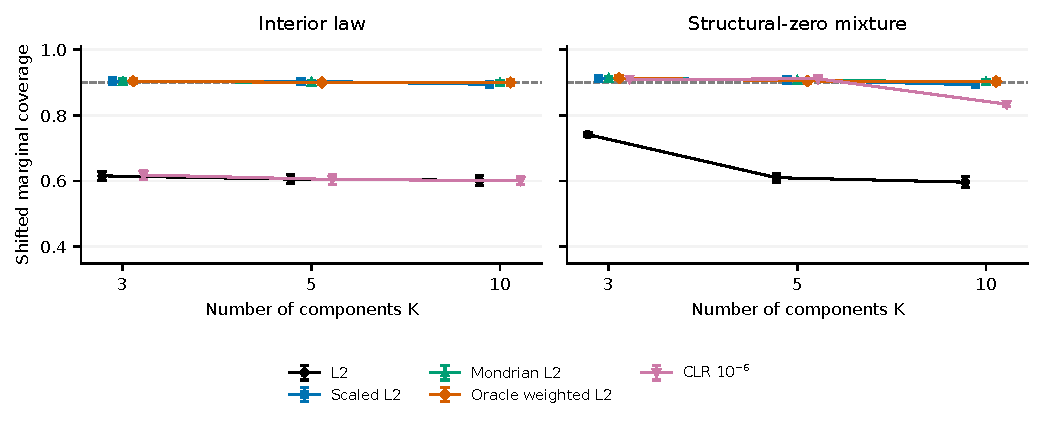
\includegraphics[width=\textwidth]{figures/shift.pdf}
\caption{Dimension-resolved shifted marginal coverage for five diagnostic comparators, with pointwise descriptive 95\% seed-bootstrap intervals. The difficult-group frequency changes from $0.2$ to $0.8$ with within-group laws preserved. CLR $10^{-6}$ in the mixture fails at $K=10$ despite near-nominal low-dimensional results; scaling also has small $K=10$ shortfalls. Complete all-method source and shift results are in Appendices~\ref{app:source}--\ref{app:shift}.}
\label{fig:shift}
\end{figure*}

\subsection{Shift, all frozen effects, and dimension heterogeneity}
Table~\ref{tab:shift} shows ordinary L2 shifted marginal coverage near $0.629$ across all six cells, versus about $0.904$ for oracle weighting and Mondrian. P3 is the L2 shifted-minus-source loss, $-0.272042$ [$-0.276837,-0.267277$]. P4, weighted-minus-ordinary shifted coverage, is $0.275410$ [$0.269120,0.281815$]. Changing the prevalence of an undercovered observable group explains the direction; target recalibration was not performed. Weighting still leaves difficult-group coverage about $0.880$ and supplies no nominal boundary guarantee.

Table~\ref{tab:contrasts} reports every frozen effect, including the size effects' different signs. P5 (Mondrian-minus-L2 shifted difficult coverage) is $0.365884$ [$0.357426,0.374758$]; P6 (scaled-minus-L2 source difficult coverage) is $0.366979$ [$0.358596,0.375569$], each averaging both laws. P9 shows that scaling \emph{reduces} source $E_Q$: $-0.095820$ [$-0.101595,-0.089812$]. There is no unavoidable efficiency-cost result. In contrast, P10 increases shifted $E_Q$ for Mondrian versus the severely undercovered ordinary L2 comparator by $0.237566$ [$0.229339,0.246762$]. All ten adjusted intervals exclude zero; this is not evidence that all directions were beneficial or all cells succeeded.

Dimension averages conceal important limitations (Figure~\ref{fig:shift}). CLR $10^{-6}$ mixture shifted coverage is $0.909160$, $0.910880$, and $0.833740$ [$0.826540,0.840810$] at $K=3,5,10$; the last cell's boundary coverage is $0.547832$ [$0.526602,0.568594$]. Scaling's $K=10$ shifted coverage is $0.894260$ [$0.889140,0.899200$] for the interior law and $0.892850$ [$0.887720,0.897610$] for the mixture. Its source difficult-group rates in those cells are $0.891134$ and $0.890417$. These are descriptive diagnostics, not additional multiplicity-adjusted tests. No universal shift-robustness claim follows from favorable averages.

\section{Discussion and Limitations}
\label{sec:limitations}
The audit changes what can be concluded, not which score universally wins. Reporting marginal coverage and ambient mass alone would omit both pooled L2's difficult-group deficit and CLR's boundary exclusion. Adding face mass does not solve the decision problem: $Q$ is an explicit convention, not an intrinsic utility. In the existing sensitivity components, Hellinger has lower source-mixture mass than Bonferroni at $\rho=0.25$ ($0.243297$ versus $0.289446$), but higher mass at $\rho=0.75$ ($0.444169$ versus $0.367424$). This exploratory ranking reversal requires no new fitting or confirmatory test (Figure~\ref{fig:sensitivity}).

The benchmark covers two synthetic laws, one exact-zero face, three dimensions, one train-only ridge predictor, $\alpha=0.1$, and a group-frequency shift with unusually transparent overlap. It has no real-data validation, multi-face/vertex response model, count or measurement-error layer, estimated density ratio, or arbitrary concept shift. Boundary status is unavailable before observing the response. The mathematical argument for transported Mondrian coverage requires preserved \emph{within-group joint} laws, while oracle weighting uses invariant $Y\mid X$ and the correct ratio. Neither justifies latent-probability, pointwise, or response-boundary nominal coverage.

Numerical resolution further limits efficiency interpretation. The pilot did not achieve uniform $0.01$ precision; zero face hits do not prove empty face intersections, and near-one ambient estimates do not prove whole-simplex regions. Bootstrap intervals quantify repeated-seed mean uncertainty, not every fitted region's MC error, a distribution over arbitrary tasks, or exact familywise control. Full per-seed face components and subgroup denominators accompany the short tables; a whole-simplex-fraction diagnostic was not recorded. Future separately frozen work should add multiple supported faces and vertices, higher-resolution face probes, other learners, and shifts within groups or estimated weighting. These are extensions, not completed experiments.

\section{Conclusion}
\label{sec:conclusion}
For observed compositions, conformal marginal coverage, conditional reliability diagnostics, and geometric reference mass answer different questions. A closed-set control proves that ambient volume alone can miss a supported face, and the completed benchmark shows why group and boundary diagnostics should remain visible alongside all reference components. Group-focused calibration can redistribute errors toward boundary responses; source scaling need not increase size; and aggregate shift recovery does not imply uniform or arbitrary-shift validity. The resulting contribution is a bounded, reproducible evaluation synthesis, not a new validity claim or a universally preferred conformal geometry.
\label{main-end}

% Flush main-body floats before the non-main-body impact statement/references.
\clearpage
\section*{Impact Statement}
This work studies reliability evaluation for synthetic compositional responses. No personal data, human participants, or deployed decision systems are used. A potential benefit is to discourage treating small geometric regions or population-average coverage as sufficient evidence of reliability for affected subpopulations. A corresponding risk is overinterpreting an arbitrary face-weighted reference measure as utility, or transferring observed-response coverage to latent probabilities or real-world groups without supporting assumptions. We explicitly separate these objects and report adverse subgroup outcomes. The synthetic results do not establish deployment safety, fairness for demographic groups, or suitability for a high-stakes application.

\bibliography{references}
\bibliographystyle{template/icml2026}

\clearpage
\appendix
\onecolumn

\section{Proofs and Exact Control Values}
\label{app:proofs}
Throughout, $T$ includes all independent training data, fitting randomness, fitted predictors, training-only scales, and fixed smoothing choices. Scores are jointly measurable and finite on the original closed simplex. Probability statements conditional on $T$ hold for almost every training realization, averaging over calibration and new-test randomness. They are not guarantees conditional on realized calibration scores. Geometry statements concern $K\geq3$ and intrinsic measures in the simplex's affine hull; $K$-dimensional Lebesgue measure of the entire simplex would be zero and is not the quantity used here.

\subsection{Corrected ranks, ties, and transformed scores}
\begin{proof}[Proof of Proposition~\ref{prop:split}]
Set $N=m+1$. Conditional on $T$, append an independent continuous uniform tie-breaking variable to each of the $N$ exchangeable scores and order pairs lexicographically. The resulting test rank $J$ is uniform on $\{1,\ldots,N\}$: exchangeability gives each index the same chance of each unique rank. If $k\leq m$ and $J\leq k$, at most $k-1$ calibration scores are strictly less than the test score, so the $k$th calibration score is at least the test score. Weak membership therefore has probability at least $k/N$. If $k=N$, the threshold is infinity and the region is the entire simplex, with coverage one. This includes $m=0$. Finally $\lceil N(1-\alpha)\rceil/N\geq1-\alpha$. Tie-breaking is a proof device, not randomness added to the implemented region.

If all $N$ scores are distinct almost surely, membership is equivalent to $J\leq k$ (also for $k=N$). Coverage then equals $k/N<1-\alpha+1/N$. Conditional i.i.d. atomless scores suffice, but continuity of the score formula does not: the constant score zero is continuous and gives coverage one. Even atomless marginals under mere exchangeability do not suffice: all scores can equal one shared continuous random variable and tie surely.
\end{proof}

Strict membership can invalidate the lower bound: a constant zero score with $q=0$ would cover nothing under $s<q$. Clipping an infeasible rank to the largest calibration score also fails: with $m=1$, $\alpha=0.1$, and continuous i.i.d. scores, that rule covers with probability $1/2$, whereas the corrected infinity convention covers with probability one.

For any train-fixed measurable $h_T$ defined on every candidate $y\in\simp$, a finite score $d_T(h_T(y),a_T(x))$ is just another $s_T$. No injectivity, isometry, inverse map, or Jacobian enters the rank proof. In particular, smoothing inside the CLR score does not change the covered object from $Y$ to a latent clean composition. Choosing among scores with the same calibration outcomes would require an additional argument and is not performed.

\subsection{Coordinate and scaling consequences}
If $s_{\rm L1}=2s_{\rm TV}$, the order statistics satisfy $q_{\rm L1}=2q_{\rm TV}$, with infinity mapping to infinity. Thus the two weak sublevel sets are identical. Training-only division by $\sigma_G>0$ also creates a legitimate fixed score, without making it group-calibrated.

For coordinate $j$, apply Proposition~\ref{prop:split} to $|Y_j-f_{T,j}(X)|$ with miscoverage $\alpha/K$. Each coordinate fails with probability at most $\alpha/K$. A union bound gives failure of any coordinate at most $\alpha$; intersecting the intervals with $\simp$ cannot remove a true response satisfying every coordinate inequality. The corrected ranks at $m=499$ are 484, 490, and 495 for $K=3,5,10$. Unadjusted calibration at $\alpha$ gives only the generic lower bound $\max(0,1-K\alpha)$ for simultaneous coverage. A jointly calibrated maximum score uses one rank for the maximum residual and is not the same construction as separately calibrated coordinates.

\subsection{Null faces, closed sets, and response coverage}
\begin{proof}[Proof of Proposition~\ref{prop:geometry}]
A proper face is contained in an affine subspace of dimension below $K-1$, and hence has zero normalized $(K-1)$-dimensional Hausdorff measure on $\simp$. If two measurable sets differ only on such a face, their ambient masses agree by bounding their mass difference by the mass of the symmetric difference.

Both $A=\{y:y_K\geq1/2\}$ and $F_K$ are closed; so is their union. In a $d$-dimensional simplex, requiring barycentric coordinate $y_K\geq t$ gives the homothetic image $y=t e_K+(1-t)z$. Its volume fraction is $(1-t)^d$. At $t=1/2$, $\Udel(A)=2^{-(K-1)}$. On $F_K$, $A$ is empty and $A^+$ contains the entire face. On another face $F_j$, $j\ne K$, the same homothety gives $U_{F_j}(A)=2^{-(K-2)}$. Adding $F_K$ changes this other-face set only on $F_j\cap F_K$, of dimension $K-3<K-2$, hence of zero $U_{F_j}$ mass. Therefore
\begin{equation}
 Q(A)=\tfrac12 2^{-(K-1)}+\tfrac{K-1}{2K}2^{-(K-2)}
      =\frac{3K-2}{K2^K},\qquad Q(A^+)=Q(A)+\frac1{2K}.
\end{equation}
The sets differ exactly by $F_K$. Positive Dirichlet parameters make the interior component give that face probability zero and the structural-zero component give it probability one. Their response coverage difference is therefore $\Prob(Y\in F_K)=0.35$, under either test regime.
\end{proof}

These statements do not assert that a fitted norm-score region realizes $A$ or $A^+$. In particular, $A^+$ need not be convex. They isolate a property of the size measure, not an algorithmic improvement. $Q$ also fails to see changes on any subset of dimension below $K-2$ lying in the probed boundary. For example, with vertex $v=e_\ell$, the closed sets $D=\{y:y_\ell\leq1/2\}$ and $D\cup\{v\}$ have equal $Q$ mass, but a response atom at $v$ distinguishes their coverages. At $K=2$ the face measures are vertex atoms, so that conclusion does not apply; all studied dimensions are at least three.

Table~\ref{tab:exact-control} lists exact values, not Monte Carlo estimates. The absolute response coverage of $A$ is not its uniform volume. For ambient-group frequency $p$, writing $p_1=p$, $p_0=1-p$, it is
\begin{equation}
 c_p=0.65\sum_{g=0}^1 p_g\E_U\left[1-I_{1/2}\!\left(\kappa_g\mu_K(U),\kappa_g(1-\mu_K(U))\right)\right],
 \label{eq:cp}
\end{equation}
where $I$ is the regularized incomplete beta function. $A^+$ has coverage $c_p+0.35$. We do not replace this unevaluated expression by an invented empirical value.

\begin{table}[htbp]
\caption{Closed-set control: exact mathematical values for $A$ versus $A^+$. The supported-face mass changes from 0 to 1. Each other-face mass is unchanged. The $0.35$ response increment is exact for the specified response mixture, not a uniform-reference probability.}
\label{tab:exact-control}
\centering
\begin{tabular}{cccccc}
\toprule
$K$ & $V(A)=V(A^+)$ & Each other $A_j$ & $Q(A)$ & $Q(A^+)$ & Response increment \\
\midrule
3 & $1/4$ & $1/2$ & $7/24$ & $11/24$ & $0.35$ \\
5 & $1/16$ & $1/8$ & $13/160$ & $29/160$ & $0.35$ \\
10 & $1/512$ & $1/256$ & $7/2560$ & $27/512$ & $0.35$ \\
\bottomrule
\end{tabular}
\end{table}

For the auxiliary deletion control $R_{\rm all}=\simp$ and $R_{\rm cut}=\simp\setminus F_K$, both ambient masses equal one; supported-face mass changes from one to zero; every other face mass remains one. Thus $Q(R_{\rm cut})=1-1/(2K)$ and mixture response coverage falls from one to $0.65$. The latter set is not closed and is not a proposed prediction method; the closed-set witness above avoids depending on that distinction. At general reference weight $\rho$, either face-change control changes $Q_\rho$ mass by $(1-\rho)/K$.

\begin{table}[htbp]
\caption{Executed closed-set control: measured response coverage gain, averaging source and shifted mixture panels within seed, versus exact geometric and response increments. Only the measured column has descriptive 95\% bootstrap uncertainty. Geometric increments are analytic assignments, not MC estimates or empirical discoveries. Source: \texttt{control\_summary.csv}.}
\label{tab:controls}
\centering
\begin{tabular}{lccccc}
\toprule
$K$ & Measured coverage gain & Exact coverage gain & $\Delta V$ & $\Delta A_K$ & $\Delta E_Q$ \\
\midrule
3 & 0.351 [0.349, 0.353] & 0.350 & 0 & 1 & 0.1667 \\
5 & 0.350 [0.348, 0.352] & 0.350 & 0 & 1 & 0.1000 \\
10 & 0.351 [0.349, 0.353] & 0.350 & 0 & 1 & 0.0500 \\
\bottomrule
\end{tabular}

\end{table}

\subsection{Sharp group bound and group-frequency transport}
\begin{proof}[Proof of Proposition~\ref{prop:group}]
Let $E=\{Y\notin\R(X)\}$ and $p=\Prob(H)>0$. Total probability gives
\begin{equation}
 \Prob(E)=p\Prob(E\mid H)+(1-p)\Prob(E\mid H^c)\geq p\Prob(E\mid H).
\end{equation}
If $\Prob(E)\leq\alpha$, then $\Prob(E\mid H)\leq\min(1,\alpha/p)$, proving the coverage bound. It is sharp: if $p\geq\alpha$, allocate failures of conditional probability $\alpha/p$ inside $H$ and none outside; if $p<\alpha$, let all of $H$ fail. These allocations can be realized with an independent uniform random variable. At $p=1$ omit the null complement; at $p=0$ conditional coverage is undefined.

For Mondrian calibration, condition on $T$, the entire vector of calibration group labels, and the new point's label $G_*=g$. If $M_g$ calibration points have label $g$, their within-group pairs and the test pair are i.i.d. with common law $P((X,Y)\in\cdot\mid G=g)$. Proposition~\ref{prop:split} with $M_g$ in place of $m$ gives coverage at least $1-\alpha$, using the realized count and the infinity convention. Averaging over calibration labels proves groupwise validity. Empty groups or infeasible ranks return $\simp$; for $\alpha=0.1$, counts zero through eight have infeasible ranks.

If an independent target point in group $g$ has the same complete within-group joint law and this group has positive source probability, the identical conditional rank argument applies to the source calibration pairs and target pair. Averaging over target group frequencies proves target marginal validity. This assumes preservation of $P(X,Y\mid G)$, not merely $P(Y\mid X)$.
\end{proof}

An exact population illustration is $C_{G=0}=1$, $C_{G=1}=0.5$. Source weights $(0.8,0.2)$ give $C=0.9$, whereas target weights $(0.2,0.8)$ give $C=0.6$. These are counterexample constants, not predictions of fitted L2 performance. For the mixture boundary, $1-0.1/0.35=5/7$. Under source sampling $\Prob(G=1,B=1)=0.07<0.1$, so marginal validity alone gives a zero lower bound on that intersection.

Observable-group $0.9$ coverage still does not imply boundary $0.9$ coverage. To exhibit the logical gap, let $H=\{U_1\leq-3/7\}$, with probability $2/7$, and return $\simp\setminus F_K$ on $H$, and $\simp$ otherwise, in every observable group. Independence of $B$ gives failure $0.35(2/7)=0.1$ within each group, while boundary coverage is $5/7$ and interior coverage is one. This constructed region is not claimed to be a fitted Mondrian L2 set; it refutes an implication, without weakening the actual group theorem.

\subsection{Oracle weighted construction and proof of its fixed-score specialization}
\label{app:weighted-proof}
We invoke the standard covariate-shift construction of \citet{tibshirani2019covariateshift}, Corollary 1 and Section 2.2, rather than claim a new weighted theorem. Conditional on independent $T$, calibration pairs are i.i.d. from $P_XP_{Y\mid X}$, the independent test pair follows $\widetilde P_XP_{Y\mid X}$, $\widetilde P_X\ll P_X$, and the known finite nonnegative ratio is $w=d\widetilde P_X/dP_X$, up to a common positive constant. It is positive at the target point almost surely. For finite $S_i=s_T(X_i,Y_i)$, define
\begin{align}
 D(x)&=\sum_{i=1}^m w(X_i)+w(x),\\
 \nu_x&=\sum_{i=1}^m\frac{w(X_i)}{D(x)}\delta_{S_i}
       +\frac{w(x)}{D(x)}\delta_{+\infty},\\
 q_w(x)&=\inf\{t\in\mathbb{R}\cup\{+\infty\}:\nu_x((-\infty,t])\geq1-\alpha\}.
 \label{eq:weighted}
\end{align}
Weak membership below $q_w$ gives target marginal coverage at least $1-\alpha$. A common rescaling of all weights changes nothing. Omitting the test atom or renormalizing only the finite atoms changes the construction.

For completeness, the finite-score specialization has a short standard weighted-rank proof. Conditional on the unordered collection of $N=m+1$ pairs, the probability that pair $i$ is the target pair is $w_i/W$, where $w_i=w(X_i)$ and $W=\sum_jw_j$. This follows by symmetrizing the joint law: relative to $P^N$, placing pair $i$ in the target position multiplies density by $w_i$, and normalization divides by $W$. The statement can equivalently be made conditional on a randomly permuted ordered collection to retain labels when pairs coincide.

If pair $i$ is target, its own score is replaced by infinity in the calibration measure. Failure $S_i>q_i$ implies that weights at scores strictly below $S_i$ already sum to at least $(1-\alpha)W$. Group equal scores and order these groups increasingly. The indices for which this can occur lie in an upper tail after a cumulative weight of at least $(1-\alpha)W$; their total weight is at most $\alpha W$. Hence the conditional probability of failure, summing $w_i/W$ over those indices, is at most $\alpha$. Integrating over the unordered collection and $T$ proves the claim and allows ties. This is a proof of the cited fixed-score case, not a simplex-specific generalization requiring new assumptions. Alternatively, push forward the response to the scalar $s_T(X,Y)$: invariant $Y\mid X$ preserves its conditional score law and the same ratio $w(X)$ applies.

With all calibration scores finite, $q_w(x)=+\infty$ if and only if the test atom $a_*=w(x)/D(x)$ is strictly greater than $\alpha$. At equality the finite mass is exactly $1-\alpha$ and reaches the quantile at its largest positive-weight score. Constant weights reduce exactly to the corrected unweighted rank, including $m=0$. With $m=1$, unit weights, and $\alpha=0.1$, dropping the infinity atom instead yields continuous-score coverage $1/2$ rather than the required lower bound.

In this experiment, $1/4\leq w\leq4$ and $m=499$, so
\begin{equation}
 a_*\leq\frac{4}{499/4+4}=\frac{16}{515}<0.1.
 \label{eq:no-infinity}
\end{equation}
Thus an infinite oracle threshold is mathematically impossible in the main design with finite scores, not merely rare. L2 scores are finite and at most $\sqrt{2}$ on the simplex. The observed zero infinity rate is therefore expected. Artificial large-weight tests exercise the infinity branch; a finite radius must not be equated with failure or success of whole-simplex inclusion. Weighted effective sample size $(\sum_iw_i)^2/\sum_iw_i^2$ is only a diagnostic, not a new unweighted rank sample size. Estimated/clipped ratios, lack of overlap, and changed conditional response laws are outside this result.

\subsection{Positive-epsilon CLR is a valid score on the closed simplex}
For $\varepsilon>0$, write
\begin{equation}
 T_\varepsilon(y)_j=\log(y_j+\varepsilon)-K^{-1}\sum_{\ell=1}^K\log(y_\ell+\varepsilon).
 \label{eq:clr}
\end{equation}
Every logarithm is finite and continuous, and the coordinate sum is zero. If $T_\varepsilon(y)=T_\varepsilon(z)$, then $y_j+\varepsilon=e^c(z_j+\varepsilon)$ for one constant $c$. Summing yields $1+K\varepsilon=e^c(1+K\varepsilon)$, so $e^c=1$ and $y=z$. The transform is injective, although injectivity is not needed for split validity. The score $\norm{T_\varepsilon(y)-T_\varepsilon(f_T(x))}_2/\sqrt K$ is finite and continuous for every original candidate $y\in\simp$, including exact zeros. Its sublevel set is evaluated directly; no unconstrained inverse image, projection of a transformed ball, or deletion of boundary observations is used. The image is compact, not the entire zero-sum hyperplane. At $\varepsilon=0$ the score is undefined at zeros and is not included in the benchmark.

\section{Complete Data-Generating Process and Fitted Predictor}
\label{app:dgp}
\subsection{Response laws and distribution shift}
For each observation, independently draw $U_1,U_2\sim\operatorname{Unif}[-1,1]$ and $G\sim\operatorname{Bernoulli}(p)$. Let $X=(U_1,U_2,G)$ and, for $j=1,\ldots,K$,
\begin{align}
 \theta_j&=2\pi(j-1)/K,\\
 a_j(u)&=0.25\sin\theta_j+0.6\cos\theta_j\,u_1
       +0.6\sin\theta_j\,u_2+0.25\cos(2\theta_j)u_1u_2,\\
 \mu_j(u)&=\frac{\exp(a_j(u))}{\sum_{\ell=1}^K\exp(a_\ell(u))},
 \qquad \kappa_0=80,\quad\kappa_1=8.
\end{align}
The interior law is
\begin{equation}
 Y\mid U=u,G=g\sim\operatorname{Dirichlet}(\kappa_g\mu(u)).
\end{equation}
For the structural-zero mixture, draw $B\sim\operatorname{Bernoulli}(0.35)$ independently of $X$. At $B=0$ use the same interior distribution. At $B=1$, set $Y_K=0$ exactly and draw
\begin{equation}
 (Y_1,\ldots,Y_{K-1})\mid X,B=1
 \sim\operatorname{Dirichlet}\left(\kappa_G\frac{\mu_{1:K-1}(U)}{1-\mu_K(U)}\right).
\end{equation}
The mixture conditional mean is
\begin{equation}
 m(u)=0.65\mu(u)+0.35\left(\frac{\mu_{1:K-1}(u)}{1-\mu_K(u)},0\right),
\end{equation}
not $\mu(u)$. $G$ changes dispersion but not component means or the boundary probability. The fitted response is $Y$, not either known mean. Known generator means are used only for generator diagnostics.

Training and calibration use $p=0.2$. Independent source and target test panels use $p=0.2$ and $0.8$. $U\mid G$, $B\mid X$, $\kappa_G$, and the response formulas remain unchanged in each law considered separately. Thus the ratio equals 4 at $G=1$ and $1/4$ at $G=0$; the complete within-group joint law is preserved and boundary prevalence remains $0.35$ in both regimes. The target panel is not a reweighted subset of the source panel.

Each of the 300 cells uses 1,500 training, 499 calibration, and two independent 2,000-observation test panels. The single-face mixture is not a multi-face or vertex DGP. All distributions and observations are synthetic; no external data access, license dependency, pretrained model, or paid API is required.

\subsection{Ridge model, projection, and scale cross-fitting}
Define the nine-dimensional feature vector
\begin{equation}
 \phi(x)=(1,u_1,u_2,u_1^2,u_2^2,u_1u_2,g,gu_1,gu_2)^\top.
\end{equation}
The multiresponse coefficient matrix is
\begin{equation}
 \widehat\beta=\arg\min_\beta\left\{\frac1{n_{\rm train}}\sum_i\norm{Y_i-\phi(X_i)^\top\beta}_2^2
       +10^{-3}\sum_{r=2}^{9}\sum_{j=1}^K\beta_{rj}^2\right\}.
\end{equation}
The intercept is unpenalized. With Euclidean simplex projection $\Pi_{\simp}$, the prediction is
\begin{equation}
 f_T(x)=(1-\delta)\Pi_{\simp}(\phi(x)^\top\widehat\beta)
             +\frac{\delta}{K}\boldsymbol{1},\qquad\delta=10^{-8}.
\end{equation}
For completeness, projection of a row $v$ uses $z_j=\max(v_j-\tau,0)$, where sorted entries $v_{(1)}\geq\cdots\geq v_{(K)}$ determine
\begin{equation}
 r=\max\left\{\ell:v_{(\ell)}-\frac{\sum_{j=1}^\ell v_{(j)}-1}{\ell}>0\right\},
 \qquad \tau=\frac{\sum_{j=1}^r v_{(j)}-1}{r}.
\end{equation}
This is deterministic given the training data and guarantees a strictly positive final predictor even when the observed response is on a face.

A training-only random permutation is divided into five equal folds (300 points each). For each held-out training fold, fit the same recipe to the other four folds and predict that fold, including projection and uniform mixing. For each $g$, define
\begin{equation}
 \sigma_g=\max\left\{10^{-3},\sqrt{\frac1{n_{{\rm train},g}}\sum_{i:G_i=g}\norm{Y_i-f_{T,-\mathrm{fold}(i)}(X_i)}_2^2}\right\}.
\end{equation}
The final predictor is then fitted on all training points. Folds, penalty, floor, and smoothing are frozen. Calibration observations are used solely for thresholds. No oracle mean predictor, alternate learner, epsilon search, or test-guided revision is included.

\section{All Method Formulas and Calibration Conventions}
\label{app:methods}
For $d=y-f_T(x)$, the six fixed scalar scores are
\begin{align}
 s_{\rm TV}(x,y)&=\tfrac12\sum_j|d_j|,\\
 s_2(x,y)&=\left(\sum_jd_j^2\right)^{1/2},\\
 s_\infty(x,y)&=\max_j|d_j|,\\
 s_H(x,y)&=\left[\tfrac12\sum_j(\sqrt{y_j}-\sqrt{f_{T,j}(x)})^2\right]^{1/2},\\
 s_{{\rm CLR},\varepsilon}(x,y)&=\frac{\norm{T_\varepsilon(y)-T_\varepsilon(f_T(x))}_2}{\sqrt K},
 \qquad\varepsilon\in\{10^{-6},10^{-2}\}.
\end{align}
Each is calibrated separately using rank 450 and weak membership as in \eqref{eq:split}. The original closed-simplex response is never floored or jittered. Hellinger and both positive-epsilon CLR scores are defined at exact zeros. Linf is a single calibrated score, not an intersection of independently calibrated coordinate regions.

For the coordinate constructions, let $q_j(\eta)$ be the corrected calibration order statistic of $|Y_{ij}-f_{T,j}(X_i)|$ at miscoverage $\eta$, with the same infinity rule. Their regions are
\begin{align}
 \R_{\rm coord}(x)&=\{y\in\simp:|y_j-f_{T,j}(x)|\leq q_j(\alpha)\ \forall j\},\\
 \R_{\rm Bonf}(x)&=\{y\in\simp:|y_j-f_{T,j}(x)|\leq q_j(\alpha/K)\ \forall j\}.
\end{align}
Clipping intervals to $[0,1]$ and intersecting with $\simp$ is implicit in candidate evaluation. Coordinate-specific rank 450 applies to the unadjusted version; corrected ranks 484/490/495 apply to Bonferroni. The latter's multiplicity correction concerns coordinates \emph{inside one prediction}, and is distinct from the bootstrap adjustment across the ten research contrasts.

Training-scale L2 calibrates $s_2(x,y)/\sigma_{g(x)}$ using one pooled quantile $q_{\rm sc}$ and accepts $s_2(x,y)\leq q_{\rm sc}\sigma_{g(x)}$. Group-Mondrian L2 calibrates $s_2$ separately within $G=g$, using $M_g$ actual calibration points and $k_g=\lceil(M_g+1)(1-\alpha)\rceil$. It accepts $s_2(x,y)\leq q_g$; empty groups or infeasible ranks use infinity. These are distinct constructions, even if their empirical group rates are similar.

Oracle weighted L2 uses \eqref{eq:weighted} with $S_i=s_2(X_i,Y_i)$ and the exact ratios. Thresholds depend on the target covariate only through $G$, so the two group thresholds are cached. The weighted row is reported only under shift. Its source unit-weight equivalence is a correctness check, not an additional baseline. No estimated weights, clipping, finite-atom renormalization, or largest-score substitution is used. Ordinary pooled scalar-score and Bonferroni guarantees apply to source marginal coverage; Mondrian targets observable-group coverage and the specified group transport; oracle weighting targets shifted marginal coverage. No listed method has a general nominal guarantee given $B$ or a fixed $u$.

\section{Frozen Contrast Definitions and Statistical Estimands}
\label{app:contrasts}
All contrasts are first minus second. For each seed, average equally across $K=3,5,10$ and, where specified, both laws. S denotes source, T denotes shifted, and Z denotes the structural-zero mixture. CLR6 and CLR2 mean $\varepsilon=10^{-6}$ and $10^{-2}$. Table~\ref{tab:definitions} gives the complete frozen definitions; Table~\ref{tab:contrasts} in the main text reports all results. These target a finite average over these DGP cells, not expected performance across arbitrary scientific tasks.

\begin{table}[htbp]
\caption{All frozen research contrasts. Every row averages all three dimensions. Source and target are compared using the same source-trained/calibrated fit; method differences are paired within each cell and seed.}
\label{tab:definitions}
\centering
\begin{tabular}{lll}
\toprule
ID & Per-cell contrast & Averaging cells \\
\midrule
P1 & L2 $C_{G=0}-C_{G=1}$ & S, Z \\
P2 & L2 $C_{B=0}-C_{B=1}$ & S, Z \\
P3 & L2 $C_{\rm T}-C_{\rm S}$ & Both laws \\
P4 & Weighted L2 $C$ minus ordinary L2 $C$ & T, both laws \\
P5 & Mondrian L2 $C_{G=1}$ minus ordinary L2 $C_{G=1}$ & T, both laws \\
P6 & Scaled L2 $C_{G=1}$ minus ordinary L2 $C_{G=1}$ & S, both laws \\
P7 & CLR6 $A_K$ minus CLR2 $A_K$ & S, Z \\
P8 & Bonferroni $C$ minus unadjusted coordinate $C$ & S, both laws \\
P9 & Scaled L2 $E_Q$ minus ordinary L2 $E_Q$ & S, both laws \\
P10 & Mondrian L2 $E_Q$ minus ordinary L2 $E_Q$ & T, both laws \\
\bottomrule
\end{tabular}
\end{table}

If $d_{sc}$ is the paired effect in seed $s$ and a specified cell $c\in\mathcal C$, the seed value is $D_s=|\mathcal C|^{-1}\sum_cd_{sc}$ and the reported effect is $50^{-1}\sum_sD_s$. Bootstrap resamples draw 50 master-seed indices with replacement and reuse those indices for all methods, dimensions, laws, regimes, and contrasts. There are 20,000 resamples, with bootstrap seed 77331. Descriptive intervals use empirical quantiles $0.025,0.975$; adjusted contrast intervals use $0.0025,0.9975$. Common seed weights preserve pairing even though the underlying simulated datasets use separate cell streams. This is not a 300-independent-replicate analysis.

All adjusted intervals exclude zero, with no null or equivalence conclusion. Their approximate coverage is a property of bootstrap inference, not an exact FWER theorem. Extreme endpoints depend on about 50 resamples per tail and only 50 original seed vectors. No p-values, additional confirmatory contrasts, optional stopping, or one-sided tests are added. The protocol's one-percentage-point coverage and $0.01$ mass flags describe practical resolution, not equivalence margins or per-seed acceptance criteria. Cellwise patterns, intersections, epsilon-related boundary-rate differences, and reference-weight rankings beyond P1--P10 are descriptive/exploratory.

The summary code averages per-seed subgroup rates rather than pooling denominators across seeds. Each panel still has the exact empirical identity $\widehat C=\sum_h(n_h/n)\widehat C_h$ for an exhaustive partition. Separately averaged subgroup rates and random prevalence estimates need not reproduce that identity by multiplying their separate means. Missing boundary groups in the interior law are not applicable, not perfect coverage.

\section{Technical Reproducibility, Monte Carlo, and Resource Details}
\label{app:technical}
\subsection{Data flow, seeds, and artifact inventory}
The local freeze manifest records \texttt{2026-11-02T20:18:00.281547+00:00}. The snapshot contains the prospective plan, configuration, implementation, and tests, with file hashes. This records local provenance, not independent verification of registration chronology. Fifty main master seeds are 1000 through 1049 inclusive; pilot seeds 900001 and 900002 are disjoint. The pilot completed 12 cells with unchanged default settings, and the main completed 300 cells. Each cell contributes ten source and eleven shifted method rows, totaling 6,300.

The implementation uses NumPy \texttt{SeedSequence([seed,K,law,stream])}, where the law indicator is zero for interior and one for the mixture. Stream indices are 0 for training, 1 for calibration, 2 for source test, 3 for target test, 5 for training cross-fitting, and $20+\mathrm{pool}$ for probes. Pool 0 is the main probe pool and pool 1 is used for independent pilot comparisons. Methods share data and probes within a cell. Cells/laws use distinct streams; inference nevertheless clusters the entire master-seed vector as frozen. Probe candidates are not used as response test observations, and no test membership enters fitting or calibration.

The following files accompany the source manuscript; relative paths are from the project root.
\begin{itemize}
\item \texttt{plan.md}, \texttt{config.json}, \texttt{preregistration/manifest.json}, and \texttt{deviations.md}: prospective choices, frozen settings, provenance, and execution deviations.
\item \texttt{experiment.py}, \texttt{test\_experiment.py}, \texttt{qa.py}, \texttt{analyze.py}, and \texttt{plot.py}: DGP/membership, correctness, pilot diagnostics, bootstrap/tables, and all manuscript figures, respectively.
\item \texttt{artifacts/main/metrics.csv}: per-seed coverage numerators and denominators, $G$ and $B$ rates/counts, all four $G\times B$ intersection rates/counts, all individual $A_j$, reference sensitivity components, predictor errors, ESS, and infinity indicators.
\item \texttt{artifacts/main/controls.csv}, \texttt{runs.csv}, and per-cell JSON and \texttt{\detokenize{*_fit.npz}} files: control membership, resource summaries, calibrated thresholds/scales, and fitted coefficients. Checkpointed cells are reused rather than replaced by new seeds.
\item \texttt{artifacts/analysis/summary\_cells.csv}, \texttt{summary\_by\_law.csv}, \texttt{summary\_overall.csv}, \texttt{contrasts.csv}, and \texttt{contrast\_seed\_values.csv}: full-precision analysis and paired effects. Short summary CSVs do not themselves contain every individual-face/intersection diagnostic; those are in the raw companion metrics.
\item \texttt{artifacts/pilot/independent\_MC.csv} and \texttt{generator\_diagnostics.csv}: independent-pool precision and generator-only checks. \texttt{pilot\_gate.md}, \texttt{artifacts\_tests.log}, and \texttt{run\_summary.json} document gates and completion.
\end{itemize}

\subsection{Matched geometric Monte Carlo}
For each group $g$, draw 64 fresh uniform covariates from $U\mid G=g$. At each, draw 512 independent $\operatorname{Dirichlet}(1,\ldots,1)$ full-simplex probes. For each $j$, draw 256 probes by setting coordinate $j$ exactly to zero and drawing the remaining $K-1$ coordinates from $\operatorname{Dirichlet}(1,\ldots,1)$. Normalized independent exponential variables implement these uniform laws. All methods see identical candidates and covariates within the cell. Membership is evaluated by its exact score inequality, not grid inversion. Numerical calculations use float64 and are streamed rather than storing all membership tensors.

For groupwise estimates $\widehat V_g,\widehat A_{jg}$, define source estimates $0.8\widehat V_0+0.2\widehat V_1$ and target estimates $0.2\widehat V_0+0.8\widehat V_1$, and analogously for each face. Then combine the stratified masses using \eqref{eq:mass}. This analytically integrates the known \emph{covariate mixture}, not the unknown response coverage. Response coverage remains an independent 2,000-observation test estimate. Sensitivity uses $E_\rho=\rho V+(1-\rho)K^{-1}\sum_jA_j$ at the three frozen values; no additional probe pools are generated for this sensitivity.

The independent pilot pools' mean absolute source differences were $0.006211$ for $V$, $0.008693$ for $A_K$, and $0.004206$ for $E_Q$; maxima were $0.023700$, $0.070068$, and $0.020468$. These did not meet a uniform $0.01$ cellwise goal. The protocol allowed retaining defaults with an MC-limited qualification, which was the recorded decision; no ranking was used to choose resolution. The main half-block diagnostic divides the 64 group covariates into two blocks of 32. For source-mixture CLR6, mean absolute block difference in $A_K$ was $0.058653$. This is a different diagnostic from two independently generated complete pools, not an error bound or a contradiction of the narrower across-seed mean interval.

Membership indicators share fitted regions and covariates and cannot be counted as independent inferential replicates. Independent seed-level test/probe randomness enters the bootstrap distribution. It does not control all numerical bias, certify $0.01$ resolution in each cell, or make all-zero hits exact zeros. The run summary records 588 all-zero supported-face rows, zero all-zero ambient-volume rows, and maximum infinite-threshold rate zero. Zero-hit rows remain in the analysis. In particular, the interior-law CLR6 supported-face estimate of zero is an MC outcome with no boundary response population to cover, not a proof that the region never touches the face. A whole-simplex-fraction diagnostic was not recorded; rounded near-one mass or a finite threshold cannot substitute for it.

\subsection{Quality checks, denominators, and operational limits}
The generator checks simplex sums to absolute tolerance $10^{-12}$ and verifies exact equality of $Y_K=0$ with the assigned $B$ flag. Normalized gamma sampling raises an exception on any unintended nonpositive gamma draw. Predictor projection and the uniform mixture ensure nonnegative, normalized predictions with positive entries. Correctness tests exercise the infeasible-rank convention, empty calibration case, constant-weight equivalence, high-weight infinity, equality $a_*=\alpha$, TV/L1 membership identity, finite zero-boundary scores, all/empty membership, and the closed-set control. The initial test log reports six passing unittest methods. Final delivery adds a seventh method testing the empty weighted-calibration endpoint: a post-review helper repair returns infinity when only the test atom remains. This branch is unreachable in the fixed main design ($m=499$); all 300 main cells were replayed with the repaired helper and matched the original numerical metrics. The original implementation and tests remain in the frozen snapshot. The unavailable \texttt{pytest} dependency was replaced by standard-library \texttt{unittest}, without changing scientific settings.

Independent generator-only samples of 100,000 per dimension/law had maximum absolute componentwise mean residual at most $0.00058219$ against the correct conditional mean. Mixture boundary prevalences were $0.34883$, $0.35032$, and $0.35036$ for $K=3,5,10$, respectively. Their easy/difficult dispersion summaries preserve the intended higher difficult-group dispersion. These checks are stochastic sanity checks, not exact proofs of a numerical generator. Actual calibration difficult-group counts ranged from 79 to 128. Test subgroup counts fluctuate: expected source counts are 400 difficult, 700 boundary, and 140 difficult-boundary observations in mixture panels of 2,000. Those are exact expectations, not observed count summaries; actual per-panel counts and coverage numerators accompany the raw metrics. Small intersections are diagnostic only and are not calibrated as separate groups.

Analysis checks the complete seed set, unique seed/dimension/law records, expected row counts, and nonmissing primary metrics. No failed seed was silently replaced or unfavorable cell excluded in the completed manifest. The manuscript-level audit reads existing artifacts; it is not an independent numerical reproduction of every RNG stream or a certification of all failure logs. Sources, freeze chronology, and whole-simplex fractions should not be described more strongly than those records support.

\subsection{Environment and measured resource fields}
The recorded environment is Python 3.11.15 on Linux x86\_64 (glibc 2.41), NumPy 2.4.6, SciPy 1.17.1, pandas 3.0.6, and Matplotlib 3.11.2. Four worker processes were used, with one BLAS thread per worker; no GPU, CUDA, neural-model dependency, or network service was used. The environment reports 40 CPUs, but a restricted cgroup inspection did not establish reserved CPU quota. Reported host memory and free disk are instantaneous availability reports, not allocations guaranteed to this job.

\begin{table}[htbp]
\caption{Operational diagnostics from the executed main run. Cell elapsed times and peak worker RSS are not summed CPU-core time or total concurrent memory. ESS is computed from calibration weights, not a substitute rank sample size.}
\label{tab:resources}
\centering
\begin{tabular}{lc}
\toprule
Field & Recorded value \\
\midrule
Completed cells / method-regime rows & 300 / 6,300 \\
Main-run wall time & 51.263 seconds \\
Sum of cell elapsed times & 195.792 seconds \\
Median / maximum cell elapsed time & 0.478 / 3.089 seconds \\
Maximum reported worker peak RSS & 78,440 KB \\
Mean weighted calibration ESS & 153.817 \\
Minimum / maximum ESS & 137.370 / 176.576 \\
Minimum / maximum calibration $G=1$ count & 79 / 128 \\
Maximum observed infinity rate & 0.0 \\
\bottomrule
\end{tabular}

\end{table}

Table~\ref{tab:resources} does not include every environment inspection, correctness test, pilot, bootstrap, plotting, or manuscript-preparation cost. Pilot cell times were about $0.114$--$0.545$ seconds and the unchanged launch projection was below the protocol's resource ceiling; these small synthetic computations need no GPU. The peak RSS is a per-worker high-water mark, not the memory of all concurrent workers. A measured main wall time is not a promised reproduction runtime on another host. The pilot gate projects stored research artifacts below 100 MB and records compliance with the 10 GB storage budget; no precise total source/PDF bundle size is claimed here.

\subsection{Reproduction commands and figure/table provenance}
The following commands describe the supplied offline pipeline. They are reproduction instructions, not claims that manuscript preparation reran the study. Run from the project root with the recorded environment; existing per-cell checkpoints are reused. Their filenames do not validate configuration/source hashes, so do not change settings and resume the same artifact directory. To force independent recomputation without destroying the supplied evidence, copy the source tree into a separate directory without its generated artifact directories first; the supplied \texttt{reproduce.py} does this safely.
\begin{verbatim}
OPENBLAS_NUM_THREADS=1 OMP_NUM_THREADS=1 MKL_NUM_THREADS=1 \
  python -m unittest -v test_experiment
OPENBLAS_NUM_THREADS=1 OMP_NUM_THREADS=1 MKL_NUM_THREADS=1 \
  python experiment.py --mode pilot --workers 4 > pilot.log 2>&1
OPENBLAS_NUM_THREADS=1 OMP_NUM_THREADS=1 MKL_NUM_THREADS=1 \
  python qa.py > qa.log 2>&1
OPENBLAS_NUM_THREADS=1 OMP_NUM_THREADS=1 MKL_NUM_THREADS=1 \
  python experiment.py --mode main --workers 4 > main.log 2>&1
python analyze.py > analysis.log 2>&1
python plot.py > plotting.log 2>&1
\end{verbatim}
The correctness, pilot, generator diagnostic, main, analysis, and plotting steps correspond to the existing logs, rather than unrun scientific extensions. \texttt{analyze.py} generates the main source coverage, source size, shift, contrast, and control table inputs and both full cell-table files from the existing metrics. \texttt{plot.py} generates Figures~\ref{fig:audit}, \ref{fig:shift}, \ref{fig:sensitivity}, and \ref{fig:strata} from the analysis CSVs. The measured control and resource table inputs are generated by \texttt{analyze.py} from the raw control memberships and recorded run metadata; the separate exact rational-geometry table is specified analytically in \texttt{paper.tex}. Bibliographic metadata and read versions are preserved in \texttt{references.bib} and \texttt{literature\_notes.md}; template provenance and unmodified official assets are in \texttt{template\_provenance.md} and \texttt{template/}.

\section{Reference Sensitivity and Response-Stratum Diagnostics}
\label{app:diagnostics}
Figure~\ref{fig:sensitivity} varies only the reference weights, not the fitted regions or response law. The observed ranking reversal between Hellinger and Bonferroni shows that a scalar summary can change order under legitimate alternative conventions. It does not establish a preferred reference or a utility-optimal winner. Figure~\ref{fig:strata} keeps dimension-specific source boundary behavior visible; pooled L2's average interior/boundary gap is not uniform, and CLR6 versus CLR2 boundary differences are particularly small at $K=3$ without implying equivalence.

\begin{figure}[htbp]
\centering
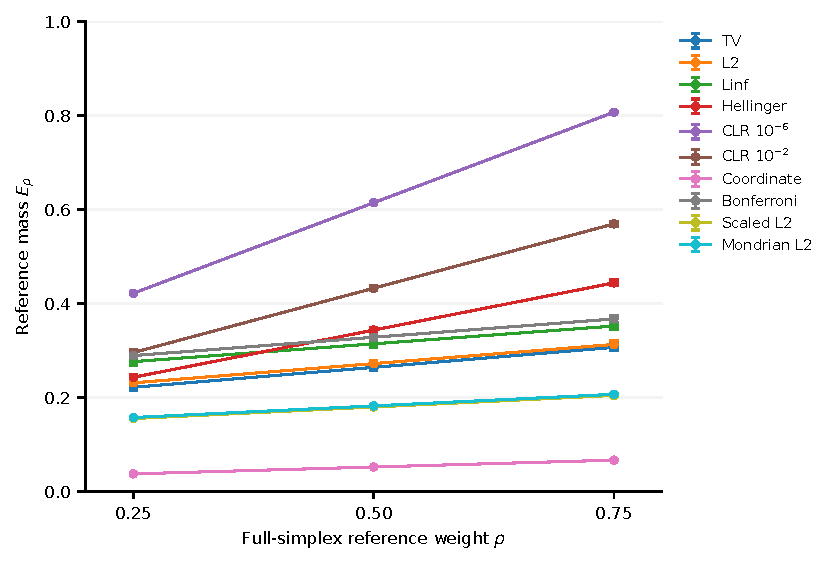
\includegraphics[width=0.82\textwidth]{figures/sensitivity.pdf}
\caption{Exploratory source-mixture reference sensitivity for all ten nonoracle methods, using the frozen $\rho$ values and existing components. Vertical bars are descriptive pointwise 95\% seed-bootstrap intervals. $E_\rho$ is normalized reference mass, not response coverage or application utility; no reference weight was selected after seeing rankings.}
\label{fig:sensitivity}
\end{figure}

\begin{figure}[htbp]
\centering
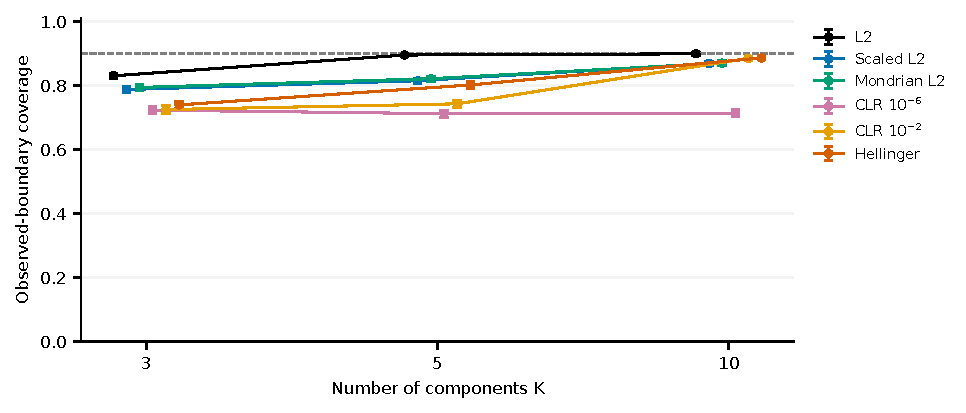
\includegraphics[width=0.90\textwidth]{figures/strata.pdf}
\caption{Source-mixture observed-boundary coverage by dimension for six diagnostic comparators. Bars are descriptive pointwise 95\% seed-bootstrap intervals; the dashed $0.9$ line is a reference target, not a guarantee conditional on boundary status. All methods and dimensions remain in the full source tables.}
\label{fig:strata}
\end{figure}

\clearpage
\section{Complete Source Results by Dimension and Law}
\label{app:source}
The following six tables retain every nonoracle method for every source DGP cell. Entries are means [pointwise descriptive 95\% CI] over the same 50 seed vectors. $C$ is simultaneous observed-composition coverage, $C_{G=1}$ is difficult-group coverage, and $C_{B=1}$ is realized-boundary coverage. Dashes indicate a nonexistent boundary-response stratum in the interior law. $V$, $A_K$, and $E_Q$ are normalized reference masses. Rounded zero/one estimates remain finite MC outcomes, not exact emptiness/whole-simplex claims; in particular near-saturated CLR ambient estimates are not exact one. Full-precision values are in \texttt{summary\_cells.csv}. All $A_j$ and intersection rates/counts remain available in \texttt{artifacts/main/metrics.csv}, beyond the selected columns printed here.
\subsection{Source, interior, $K=3$}

\begin{center}\scriptsize\resizebox{\textwidth}{!}{%
\begin{tabular}{lcccccc}
\toprule
Method & $C$ & $C_{G=1}$ & $C_{B=1}$ & $V$ & $A_K$ & $E_Q$ \\
\midrule
TV & 0.900 [0.896, 0.904] & 0.512 [0.494, 0.530] & -- & 0.186 [0.178, 0.194] & 0.044 [0.039, 0.048] & 0.103 [0.098, 0.108] \\
L2 & 0.900 [0.896, 0.905] & 0.512 [0.493, 0.531] & -- & 0.186 [0.178, 0.194] & 0.043 [0.039, 0.048] & 0.103 [0.098, 0.108] \\
Linf & 0.900 [0.896, 0.904] & 0.512 [0.494, 0.530] & -- & 0.186 [0.178, 0.194] & 0.044 [0.039, 0.048] & 0.103 [0.098, 0.108] \\
Hellinger & 0.901 [0.897, 0.905] & 0.508 [0.492, 0.525] & -- & 0.191 [0.183, 0.199] & 0.000 [0.000, 0.000] & 0.096 [0.092, 0.100] \\
CLR $10^{-6}$ & 0.902 [0.898, 0.906] & 0.518 [0.501, 0.536] & -- & 0.210 [0.201, 0.219] & 0.000 [0.000, 0.000] & 0.105 [0.101, 0.110] \\
CLR $10^{-2}$ & 0.901 [0.897, 0.905] & 0.514 [0.497, 0.531] & -- & 0.206 [0.198, 0.215] & 0.000 [0.000, 0.000] & 0.103 [0.099, 0.108] \\
Coordinate & 0.821 [0.815, 0.826] & 0.288 [0.276, 0.300] & -- & 0.091 [0.088, 0.095] & 0.006 [0.005, 0.007] & 0.047 [0.046, 0.049] \\
Bonferroni & 0.929 [0.927, 0.932] & 0.650 [0.636, 0.663] & -- & 0.259 [0.251, 0.267] & 0.081 [0.074, 0.088] & 0.151 [0.146, 0.157] \\
Scaled L2 & 0.899 [0.895, 0.904] & 0.905 [0.899, 0.911] & -- & 0.151 [0.149, 0.153] & 0.058 [0.056, 0.060] & 0.095 [0.093, 0.097] \\
Mondrian L2 & 0.901 [0.896, 0.906] & 0.902 [0.890, 0.912] & -- & 0.152 [0.149, 0.155] & 0.059 [0.056, 0.062] & 0.096 [0.093, 0.098] \\
\bottomrule
\end{tabular}
}\end{center}

\subsection{Source, interior, $K=5$}

\begin{center}\scriptsize\resizebox{\textwidth}{!}{%
\begin{tabular}{lcccccc}
\toprule
Method & $C$ & $C_{G=1}$ & $C_{B=1}$ & $V$ & $A_K$ & $E_Q$ \\
\midrule
TV & 0.901 [0.897, 0.904] & 0.505 [0.490, 0.521] & -- & 0.215 [0.206, 0.225] & 0.102 [0.095, 0.109] & 0.143 [0.136, 0.150] \\
L2 & 0.901 [0.897, 0.905] & 0.506 [0.488, 0.523] & -- & 0.210 [0.200, 0.221] & 0.105 [0.097, 0.113] & 0.139 [0.132, 0.147] \\
Linf & 0.903 [0.900, 0.906] & 0.515 [0.499, 0.531] & -- & 0.234 [0.223, 0.246] & 0.135 [0.125, 0.144] & 0.164 [0.155, 0.173] \\
Hellinger & 0.902 [0.898, 0.906] & 0.510 [0.492, 0.529] & -- & 0.220 [0.211, 0.230] & 0.008 [0.006, 0.010] & 0.112 [0.107, 0.117] \\
CLR $10^{-6}$ & 0.900 [0.896, 0.905] & 0.503 [0.482, 0.523] & -- & 0.274 [0.259, 0.290] & 0.000 [0.000, 0.000] & 0.137 [0.130, 0.145] \\
CLR $10^{-2}$ & 0.900 [0.896, 0.904] & 0.499 [0.480, 0.518] & -- & 0.252 [0.239, 0.264] & 0.00003 [0.00001, 0.00006] & 0.126 [0.120, 0.132] \\
Coordinate & 0.737 [0.731, 0.744] & 0.092 [0.085, 0.098] & -- & 0.026 [0.025, 0.028] & 0.005 [0.005, 0.006] & 0.014 [0.014, 0.015] \\
Bonferroni & 0.916 [0.913, 0.918] & 0.580 [0.567, 0.592] & -- & 0.282 [0.272, 0.292] & 0.165 [0.156, 0.175] & 0.203 [0.194, 0.211] \\
Scaled L2 & 0.902 [0.897, 0.906] & 0.905 [0.899, 0.912] & -- & 0.141 [0.139, 0.144] & 0.097 [0.095, 0.100] & 0.111 [0.109, 0.114] \\
Mondrian L2 & 0.904 [0.900, 0.908] & 0.901 [0.891, 0.911] & -- & 0.140 [0.137, 0.144] & 0.096 [0.092, 0.100] & 0.110 [0.106, 0.114] \\
\bottomrule
\end{tabular}
}\end{center}

\subsection{Source, interior, $K=10$}

\begin{center}\scriptsize\resizebox{\textwidth}{!}{%
\begin{tabular}{lcccccc}
\toprule
Method & $C$ & $C_{G=1}$ & $C_{B=1}$ & $V$ & $A_K$ & $E_Q$ \\
\midrule
TV & 0.898 [0.893, 0.903] & 0.490 [0.469, 0.511] & -- & 0.482 [0.464, 0.500] & 0.346 [0.329, 0.363] & 0.403 [0.386, 0.420] \\
L2 & 0.901 [0.896, 0.905] & 0.503 [0.481, 0.524] & -- & 0.512 [0.490, 0.532] & 0.391 [0.370, 0.411] & 0.438 [0.418, 0.459] \\
Linf & 0.900 [0.896, 0.905] & 0.502 [0.481, 0.522] & -- & 0.570 [0.550, 0.590] & 0.480 [0.459, 0.500] & 0.520 [0.499, 0.541] \\
Hellinger & 0.899 [0.895, 0.904] & 0.496 [0.477, 0.515] & -- & 0.533 [0.517, 0.549] & 0.230 [0.215, 0.244] & 0.364 [0.350, 0.378] \\
CLR $10^{-6}$ & 0.900 [0.896, 0.904] & 0.500 [0.482, 0.518] & -- & 0.774 [0.758, 0.789] & 0.000 [0.000, 0.000] & 0.387 [0.379, 0.394] \\
CLR $10^{-2}$ & 0.898 [0.894, 0.902] & 0.490 [0.471, 0.508] & -- & 0.530 [0.516, 0.543] & 0.182 [0.170, 0.195] & 0.339 [0.327, 0.350] \\
Coordinate & 0.577 [0.570, 0.584] & 0.005 [0.004, 0.006] & -- & 0.0039 [0.0036, 0.0042] & 0.0010 [0.0009, 0.0011] & 0.002 [0.002, 0.003] \\
Bonferroni & 0.905 [0.901, 0.909] & 0.526 [0.509, 0.543] & -- & 0.571 [0.553, 0.589] & 0.489 [0.470, 0.508] & 0.524 [0.505, 0.542] \\
Scaled L2 & 0.896 [0.892, 0.901] & 0.891 [0.885, 0.898] & -- & 0.185 [0.184, 0.186] & 0.172 [0.171, 0.174] & 0.177 [0.176, 0.178] \\
Mondrian L2 & 0.898 [0.894, 0.902] & 0.896 [0.885, 0.906] & -- & 0.186 [0.184, 0.188] & 0.174 [0.171, 0.176] & 0.178 [0.176, 0.181] \\
\bottomrule
\end{tabular}
}\end{center}

\subsection{Source, zeros, $K=3$}

\begin{center}\scriptsize\resizebox{\textwidth}{!}{%
\begin{tabular}{lcccccc}
\toprule
Method & $C$ & $C_{G=1}$ & $C_{B=1}$ & $V$ & $A_K$ & $E_Q$ \\
\midrule
TV & 0.903 [0.899, 0.906] & 0.693 [0.684, 0.702] & 0.830 [0.821, 0.839] & 0.345 [0.340, 0.350] & 0.321 [0.315, 0.328] & 0.237 [0.234, 0.241] \\
L2 & 0.902 [0.898, 0.906] & 0.685 [0.676, 0.695] & 0.829 [0.821, 0.838] & 0.339 [0.334, 0.343] & 0.320 [0.314, 0.327] & 0.233 [0.230, 0.237] \\
Linf & 0.903 [0.899, 0.906] & 0.693 [0.684, 0.702] & 0.830 [0.821, 0.839] & 0.345 [0.340, 0.350] & 0.321 [0.315, 0.328] & 0.237 [0.234, 0.241] \\
Hellinger & 0.904 [0.900, 0.909] & 0.856 [0.849, 0.864] & 0.739 [0.728, 0.750] & 0.662 [0.657, 0.668] & 0.399 [0.388, 0.410] & 0.405 [0.400, 0.409] \\
CLR $10^{-6}$ & 0.903 [0.898, 0.907] & 0.907 [0.900, 0.914] & 0.723 [0.711, 0.735] & 0.999991 [0.999987, 0.999995] & 0.788 [0.774, 0.801] & 0.656 [0.653, 0.660] \\
CLR $10^{-2}$ & 0.903 [0.898, 0.908] & 0.898 [0.890, 0.905] & 0.724 [0.712, 0.737] & 0.895 [0.892, 0.898] & 0.589 [0.573, 0.604] & 0.555 [0.550, 0.559] \\
Coordinate & 0.795 [0.789, 0.801] & 0.448 [0.438, 0.458] & 0.646 [0.635, 0.656] & 0.198 [0.195, 0.201] & 0.164 [0.160, 0.168] & 0.129 [0.127, 0.131] \\
Bonferroni & 0.926 [0.922, 0.929] & 0.706 [0.695, 0.718] & 0.887 [0.879, 0.894] & 0.351 [0.344, 0.357] & 0.329 [0.321, 0.338] & 0.241 [0.236, 0.247] \\
Scaled L2 & 0.904 [0.900, 0.908] & 0.916 [0.909, 0.923] & 0.787 [0.777, 0.797] & 0.327 [0.322, 0.332] & 0.300 [0.293, 0.306] & 0.228 [0.224, 0.232] \\
Mondrian L2 & 0.907 [0.903, 0.911] & 0.915 [0.906, 0.924] & 0.793 [0.783, 0.803] & 0.331 [0.326, 0.335] & 0.304 [0.298, 0.311] & 0.231 [0.228, 0.235] \\
\bottomrule
\end{tabular}
}\end{center}

\subsection{Source, zeros, $K=5$}

\begin{center}\scriptsize\resizebox{\textwidth}{!}{%
\begin{tabular}{lcccccc}
\toprule
Method & $C$ & $C_{G=1}$ & $C_{B=1}$ & $V$ & $A_K$ & $E_Q$ \\
\midrule
TV & 0.900 [0.896, 0.904] & 0.502 [0.486, 0.518] & 0.892 [0.887, 0.898] & 0.225 [0.215, 0.235] & 0.176 [0.167, 0.184] & 0.154 [0.147, 0.162] \\
L2 & 0.901 [0.897, 0.905] & 0.512 [0.495, 0.528] & 0.894 [0.889, 0.900] & 0.223 [0.213, 0.234] & 0.188 [0.179, 0.197] & 0.155 [0.147, 0.162] \\
Linf & 0.901 [0.897, 0.905] & 0.532 [0.517, 0.546] & 0.891 [0.885, 0.897] & 0.255 [0.245, 0.265] & 0.223 [0.215, 0.232] & 0.185 [0.177, 0.193] \\
Hellinger & 0.901 [0.897, 0.905] & 0.665 [0.652, 0.678] & 0.801 [0.791, 0.811] & 0.415 [0.408, 0.423] & 0.189 [0.182, 0.196] & 0.236 [0.231, 0.241] \\
CLR $10^{-6}$ & 0.899 [0.895, 0.903] & 0.914 [0.907, 0.922] & 0.711 [0.700, 0.723] & 0.99998 [0.99997, 0.99999] & 0.766 [0.753, 0.780] & 0.619 [0.616, 0.623] \\
CLR $10^{-2}$ & 0.901 [0.897, 0.905] & 0.817 [0.809, 0.826] & 0.742 [0.732, 0.753] & 0.675 [0.669, 0.681] & 0.327 [0.316, 0.339] & 0.380 [0.376, 0.384] \\
Coordinate & 0.702 [0.696, 0.708] & 0.123 [0.117, 0.129] & 0.599 [0.589, 0.608] & 0.042 [0.040, 0.043] & 0.034 [0.032, 0.035] & 0.025 [0.025, 0.026] \\
Bonferroni & 0.914 [0.911, 0.917] & 0.589 [0.577, 0.602] & 0.906 [0.901, 0.911] & 0.301 [0.291, 0.311] & 0.266 [0.256, 0.275] & 0.224 [0.215, 0.232] \\
Scaled L2 & 0.899 [0.894, 0.903] & 0.907 [0.900, 0.914] & 0.814 [0.806, 0.822] & 0.174 [0.171, 0.177] & 0.150 [0.147, 0.153] & 0.134 [0.132, 0.137] \\
Mondrian L2 & 0.902 [0.897, 0.906] & 0.903 [0.892, 0.913] & 0.821 [0.813, 0.828] & 0.175 [0.172, 0.179] & 0.151 [0.147, 0.155] & 0.135 [0.132, 0.139] \\
\bottomrule
\end{tabular}
}\end{center}

\subsection{Source, zeros, $K=10$}

\begin{center}\scriptsize\resizebox{\textwidth}{!}{%
\begin{tabular}{lcccccc}
\toprule
Method & $C$ & $C_{G=1}$ & $C_{B=1}$ & $V$ & $A_K$ & $E_Q$ \\
\midrule
TV & 0.898 [0.893, 0.902] & 0.491 [0.469, 0.513] & 0.896 [0.891, 0.902] & 0.479 [0.460, 0.498] & 0.415 [0.396, 0.434] & 0.402 [0.384, 0.421] \\
L2 & 0.899 [0.894, 0.903] & 0.496 [0.472, 0.518] & 0.898 [0.893, 0.903] & 0.500 [0.480, 0.521] & 0.440 [0.420, 0.460] & 0.429 [0.409, 0.449] \\
Linf & 0.899 [0.895, 0.903] & 0.498 [0.477, 0.518] & 0.898 [0.893, 0.902] & 0.571 [0.550, 0.591] & 0.501 [0.481, 0.521] & 0.521 [0.500, 0.542] \\
Hellinger & 0.899 [0.895, 0.903] & 0.497 [0.476, 0.518] & 0.885 [0.880, 0.890] & 0.556 [0.538, 0.573] & 0.385 [0.366, 0.404] & 0.391 [0.375, 0.407] \\
CLR $10^{-6}$ & 0.898 [0.894, 0.902] & 0.813 [0.803, 0.823] & 0.712 [0.701, 0.723] & 0.9996 [0.9992, 0.9998] & 0.533 [0.515, 0.551] & 0.569 [0.565, 0.572] \\
CLR $10^{-2}$ & 0.898 [0.893, 0.902] & 0.492 [0.470, 0.513] & 0.884 [0.879, 0.889] & 0.550 [0.533, 0.566] & 0.373 [0.354, 0.392] & 0.364 [0.349, 0.378] \\
Coordinate & 0.556 [0.547, 0.564] & 0.006 [0.004, 0.007] & 0.497 [0.486, 0.507] & 0.0051 [0.0048, 0.0055] & 0.004 [0.003, 0.004] & 0.0032 [0.0030, 0.0034] \\
Bonferroni & 0.904 [0.900, 0.908] & 0.526 [0.508, 0.544] & 0.904 [0.899, 0.909] & 0.567 [0.549, 0.586] & 0.517 [0.499, 0.534] & 0.521 [0.502, 0.539] \\
Scaled L2 & 0.901 [0.896, 0.905] & 0.890 [0.883, 0.898] & 0.868 [0.861, 0.874] & 0.187 [0.186, 0.188] & 0.178 [0.177, 0.179] & 0.178 [0.176, 0.179] \\
Mondrian L2 & 0.902 [0.897, 0.907] & 0.905 [0.894, 0.915] & 0.869 [0.862, 0.876] & 0.189 [0.187, 0.191] & 0.181 [0.178, 0.183] & 0.181 [0.178, 0.183] \\
\bottomrule
\end{tabular}
}\end{center}


\clearpage
\section{Complete Shifted Results by Dimension and Law}
\label{app:shift}
The following six tables use the same source fits/calibration and fresh target-response panels. They include all ten nonoracle methods and the oracle-weighted comparator, with the same descriptive-interval and finite-MC conventions as Appendix~\ref{app:source}. Source and target mass columns integrate different known covariate mixtures, and should not be interpreted as same-population utility differences. Figure~\ref{fig:shift} highlights, rather than replaces, these complete dimension-resolved comparisons.
\subsection{Shift, interior, $K=3$}

\begin{center}\scriptsize\resizebox{\textwidth}{!}{%
\begin{tabular}{lcccccc}
\toprule
Method & $C$ & $C_{G=1}$ & $C_{B=1}$ & $V$ & $A_K$ & $E_Q$ \\
\midrule
TV & 0.615 [0.602, 0.628] & 0.519 [0.503, 0.535] & -- & 0.186 [0.178, 0.194] & 0.047 [0.042, 0.052] & 0.104 [0.099, 0.109] \\
L2 & 0.616 [0.602, 0.629] & 0.520 [0.503, 0.537] & -- & 0.186 [0.178, 0.194] & 0.046 [0.041, 0.052] & 0.104 [0.099, 0.109] \\
Linf & 0.615 [0.602, 0.628] & 0.519 [0.503, 0.535] & -- & 0.186 [0.178, 0.194] & 0.047 [0.042, 0.052] & 0.104 [0.099, 0.109] \\
Hellinger & 0.612 [0.599, 0.626] & 0.515 [0.498, 0.533] & -- & 0.191 [0.183, 0.199] & 0.000 [0.000, 0.000] & 0.095 [0.092, 0.099] \\
CLR $10^{-6}$ & 0.619 [0.605, 0.632] & 0.524 [0.507, 0.541] & -- & 0.209 [0.201, 0.218] & 0.000 [0.000, 0.000] & 0.105 [0.100, 0.109] \\
CLR $10^{-2}$ & 0.616 [0.603, 0.630] & 0.521 [0.504, 0.538] & -- & 0.206 [0.197, 0.214] & 0.000 [0.000, 0.000] & 0.103 [0.099, 0.107] \\
Coordinate & 0.421 [0.413, 0.429] & 0.287 [0.278, 0.297] & -- & 0.092 [0.089, 0.095] & 0.007 [0.005, 0.009] & 0.048 [0.046, 0.049] \\
Bonferroni & 0.722 [0.712, 0.733] & 0.653 [0.640, 0.666] & -- & 0.258 [0.251, 0.266] & 0.084 [0.078, 0.091] & 0.152 [0.146, 0.157] \\
Scaled L2 & 0.904 [0.899, 0.909] & 0.905 [0.900, 0.911] & -- & 0.410 [0.404, 0.417] & 0.226 [0.218, 0.235] & 0.281 [0.275, 0.287] \\
Mondrian L2 & 0.903 [0.894, 0.911] & 0.903 [0.893, 0.913] & -- & 0.411 [0.399, 0.423] & 0.229 [0.216, 0.241] & 0.282 [0.271, 0.292] \\
Weighted L2 & 0.904 [0.895, 0.912] & 0.880 [0.869, 0.890] & -- & 0.458 [0.446, 0.470] & 0.246 [0.234, 0.257] & 0.309 [0.298, 0.319] \\
\bottomrule
\end{tabular}
}\end{center}

\subsection{Shift, interior, $K=5$}

\begin{center}\scriptsize\resizebox{\textwidth}{!}{%
\begin{tabular}{lcccccc}
\toprule
Method & $C$ & $C_{G=1}$ & $C_{B=1}$ & $V$ & $A_K$ & $E_Q$ \\
\midrule
TV & 0.607 [0.593, 0.620] & 0.509 [0.492, 0.525] & -- & 0.215 [0.206, 0.225] & 0.102 [0.096, 0.109] & 0.142 [0.135, 0.150] \\
L2 & 0.606 [0.592, 0.620] & 0.508 [0.491, 0.525] & -- & 0.209 [0.199, 0.220] & 0.105 [0.098, 0.113] & 0.139 [0.131, 0.147] \\
Linf & 0.610 [0.597, 0.623] & 0.513 [0.497, 0.529] & -- & 0.233 [0.222, 0.245] & 0.135 [0.125, 0.145] & 0.163 [0.154, 0.173] \\
Hellinger & 0.608 [0.594, 0.622] & 0.511 [0.493, 0.528] & -- & 0.220 [0.210, 0.230] & 0.008 [0.006, 0.010] & 0.112 [0.106, 0.117] \\
CLR $10^{-6}$ & 0.605 [0.589, 0.621] & 0.507 [0.487, 0.526] & -- & 0.273 [0.258, 0.289] & 0.000 [0.000, 0.000] & 0.137 [0.129, 0.144] \\
CLR $10^{-2}$ & 0.602 [0.586, 0.617] & 0.503 [0.484, 0.522] & -- & 0.251 [0.238, 0.263] & 0.00010 [0.00002, 0.00023] & 0.125 [0.119, 0.132] \\
Coordinate & 0.252 [0.247, 0.257] & 0.091 [0.087, 0.095] & -- & 0.026 [0.025, 0.028] & 0.005 [0.004, 0.006] & 0.014 [0.014, 0.015] \\
Bonferroni & 0.662 [0.652, 0.672] & 0.578 [0.566, 0.590] & -- & 0.281 [0.271, 0.291] & 0.166 [0.157, 0.175] & 0.202 [0.193, 0.210] \\
Scaled L2 & 0.904 [0.899, 0.909] & 0.905 [0.899, 0.911] & -- & 0.508 [0.499, 0.518] & 0.378 [0.369, 0.388] & 0.414 [0.404, 0.424] \\
Mondrian L2 & 0.900 [0.893, 0.907] & 0.900 [0.891, 0.908] & -- & 0.502 [0.488, 0.516] & 0.372 [0.357, 0.388] & 0.408 [0.393, 0.423] \\
Weighted L2 & 0.900 [0.893, 0.907] & 0.875 [0.866, 0.884] & -- & 0.575 [0.559, 0.590] & 0.412 [0.396, 0.428] & 0.457 [0.442, 0.473] \\
\bottomrule
\end{tabular}
}\end{center}

\subsection{Shift, interior, $K=10$}

\begin{center}\scriptsize\resizebox{\textwidth}{!}{%
\begin{tabular}{lcccccc}
\toprule
Method & $C$ & $C_{G=1}$ & $C_{B=1}$ & $V$ & $A_K$ & $E_Q$ \\
\midrule
TV & 0.592 [0.577, 0.607] & 0.490 [0.471, 0.508] & -- & 0.478 [0.459, 0.496] & 0.344 [0.325, 0.362] & 0.399 [0.381, 0.416] \\
L2 & 0.602 [0.586, 0.618] & 0.503 [0.482, 0.522] & -- & 0.506 [0.485, 0.526] & 0.387 [0.365, 0.408] & 0.434 [0.413, 0.454] \\
Linf & 0.602 [0.586, 0.618] & 0.503 [0.482, 0.522] & -- & 0.568 [0.547, 0.587] & 0.479 [0.458, 0.499] & 0.518 [0.497, 0.538] \\
Hellinger & 0.600 [0.585, 0.614] & 0.500 [0.482, 0.518] & -- & 0.527 [0.510, 0.544] & 0.229 [0.213, 0.245] & 0.360 [0.346, 0.375] \\
CLR $10^{-6}$ & 0.601 [0.588, 0.614] & 0.501 [0.485, 0.517] & -- & 0.769 [0.753, 0.785] & 0.000 [0.000, 0.000] & 0.385 [0.376, 0.392] \\
CLR $10^{-2}$ & 0.595 [0.581, 0.608] & 0.494 [0.477, 0.510] & -- & 0.523 [0.508, 0.538] & 0.182 [0.169, 0.194] & 0.335 [0.322, 0.347] \\
Coordinate & 0.147 [0.144, 0.150] & 0.005 [0.004, 0.005] & -- & 0.0039 [0.0036, 0.0041] & 0.0010 [0.0009, 0.0011] & 0.002 [0.002, 0.003] \\
Bonferroni & 0.620 [0.606, 0.634] & 0.525 [0.507, 0.542] & -- & 0.569 [0.551, 0.587] & 0.488 [0.469, 0.506] & 0.522 [0.503, 0.539] \\
Scaled L2 & 0.894 [0.889, 0.899] & 0.894 [0.888, 0.899] & -- & 0.727 [0.722, 0.731] & 0.685 [0.679, 0.691] & 0.700 [0.695, 0.706] \\
Mondrian L2 & 0.899 [0.890, 0.907] & 0.899 [0.889, 0.909] & -- & 0.731 [0.723, 0.738] & 0.691 [0.681, 0.701] & 0.706 [0.696, 0.715] \\
Weighted L2 & 0.900 [0.890, 0.909] & 0.875 [0.863, 0.886] & -- & 0.887 [0.876, 0.898] & 0.830 [0.814, 0.844] & 0.851 [0.837, 0.864] \\
\bottomrule
\end{tabular}
}\end{center}

\subsection{Shift, zeros, $K=3$}

\begin{center}\scriptsize\resizebox{\textwidth}{!}{%
\begin{tabular}{lcccccc}
\toprule
Method & $C$ & $C_{G=1}$ & $C_{B=1}$ & $V$ & $A_K$ & $E_Q$ \\
\midrule
TV & 0.746 [0.741, 0.751] & 0.695 [0.689, 0.701] & 0.679 [0.669, 0.690] & 0.343 [0.338, 0.348] & 0.324 [0.317, 0.330] & 0.238 [0.234, 0.241] \\
L2 & 0.741 [0.736, 0.747] & 0.689 [0.683, 0.695] & 0.676 [0.665, 0.687] & 0.337 [0.333, 0.342] & 0.323 [0.315, 0.330] & 0.234 [0.231, 0.237] \\
Linf & 0.746 [0.741, 0.751] & 0.695 [0.689, 0.701] & 0.679 [0.669, 0.690] & 0.343 [0.338, 0.348] & 0.324 [0.317, 0.330] & 0.238 [0.234, 0.241] \\
Hellinger & 0.871 [0.866, 0.875] & 0.860 [0.854, 0.865] & 0.681 [0.668, 0.695] & 0.660 [0.653, 0.667] & 0.401 [0.389, 0.414] & 0.405 [0.400, 0.409] \\
CLR $10^{-6}$ & 0.909 [0.905, 0.914] & 0.911 [0.906, 0.916] & 0.741 [0.728, 0.755] & 0.999990 [0.999986, 0.999994] & 0.790 [0.773, 0.807] & 0.658 [0.654, 0.661] \\
CLR $10^{-2}$ & 0.903 [0.898, 0.907] & 0.902 [0.897, 0.908] & 0.724 [0.711, 0.739] & 0.894 [0.890, 0.897] & 0.592 [0.573, 0.612] & 0.556 [0.551, 0.559] \\
Coordinate & 0.532 [0.526, 0.539] & 0.447 [0.440, 0.454] & 0.425 [0.414, 0.436] & 0.198 [0.195, 0.201] & 0.166 [0.161, 0.172] & 0.129 [0.127, 0.131] \\
Bonferroni & 0.764 [0.757, 0.772] & 0.711 [0.702, 0.720] & 0.709 [0.696, 0.722] & 0.349 [0.343, 0.356] & 0.330 [0.322, 0.339] & 0.241 [0.236, 0.247] \\
Scaled L2 & 0.913 [0.908, 0.917] & 0.916 [0.910, 0.921] & 0.882 [0.874, 0.889] & 0.501 [0.492, 0.510] & 0.496 [0.488, 0.504] & 0.376 [0.369, 0.383] \\
Mondrian L2 & 0.913 [0.907, 0.919] & 0.915 [0.908, 0.923] & 0.882 [0.872, 0.891] & 0.505 [0.494, 0.516] & 0.499 [0.487, 0.510] & 0.380 [0.370, 0.390] \\
Weighted L2 & 0.913 [0.906, 0.920] & 0.892 [0.884, 0.901] & 0.906 [0.895, 0.916] & 0.525 [0.513, 0.537] & 0.526 [0.512, 0.539] & 0.393 [0.383, 0.404] \\
\bottomrule
\end{tabular}
}\end{center}

\subsection{Shift, zeros, $K=5$}

\begin{center}\scriptsize\resizebox{\textwidth}{!}{%
\begin{tabular}{lcccccc}
\toprule
Method & $C$ & $C_{G=1}$ & $C_{B=1}$ & $V$ & $A_K$ & $E_Q$ \\
\midrule
TV & 0.605 [0.592, 0.617] & 0.507 [0.491, 0.522] & 0.572 [0.557, 0.586] & 0.224 [0.214, 0.234] & 0.175 [0.167, 0.183] & 0.154 [0.146, 0.161] \\
L2 & 0.610 [0.597, 0.623] & 0.514 [0.498, 0.530] & 0.585 [0.569, 0.601] & 0.223 [0.213, 0.233] & 0.187 [0.178, 0.196] & 0.154 [0.147, 0.162] \\
Linf & 0.627 [0.617, 0.637] & 0.536 [0.523, 0.549] & 0.604 [0.593, 0.615] & 0.255 [0.245, 0.265] & 0.222 [0.213, 0.231] & 0.185 [0.177, 0.193] \\
Hellinger & 0.726 [0.719, 0.734] & 0.668 [0.659, 0.677] & 0.546 [0.532, 0.561] & 0.414 [0.405, 0.422] & 0.188 [0.181, 0.196] & 0.235 [0.230, 0.240] \\
CLR $10^{-6}$ & 0.911 [0.905, 0.916] & 0.914 [0.907, 0.921] & 0.745 [0.729, 0.761] & 0.99997 [0.99997, 0.99998] & 0.759 [0.741, 0.776] & 0.620 [0.616, 0.624] \\
CLR $10^{-2}$ & 0.835 [0.829, 0.842] & 0.813 [0.805, 0.821] & 0.631 [0.615, 0.647] & 0.672 [0.665, 0.679] & 0.325 [0.313, 0.338] & 0.379 [0.374, 0.383] \\
Coordinate & 0.271 [0.266, 0.275] & 0.128 [0.123, 0.132] & 0.233 [0.227, 0.239] & 0.042 [0.040, 0.043] & 0.033 [0.032, 0.035] & 0.025 [0.025, 0.026] \\
Bonferroni & 0.673 [0.663, 0.682] & 0.593 [0.580, 0.604] & 0.654 [0.643, 0.665] & 0.301 [0.290, 0.311] & 0.264 [0.255, 0.273] & 0.223 [0.215, 0.231] \\
Scaled L2 & 0.908 [0.903, 0.912] & 0.909 [0.903, 0.915] & 0.883 [0.877, 0.889] & 0.524 [0.515, 0.534] & 0.476 [0.467, 0.485] & 0.433 [0.423, 0.442] \\
Mondrian L2 & 0.906 [0.900, 0.912] & 0.906 [0.898, 0.914] & 0.883 [0.876, 0.890] & 0.523 [0.510, 0.536] & 0.475 [0.462, 0.488] & 0.432 [0.418, 0.446] \\
Weighted L2 & 0.905 [0.898, 0.911] & 0.881 [0.873, 0.888] & 0.899 [0.892, 0.906] & 0.591 [0.576, 0.605] & 0.533 [0.519, 0.548] & 0.479 [0.464, 0.493] \\
\bottomrule
\end{tabular}
}\end{center}

\subsection{Shift, zeros, $K=10$}

\begin{center}\scriptsize\resizebox{\textwidth}{!}{%
\begin{tabular}{lcccccc}
\toprule
Method & $C$ & $C_{G=1}$ & $C_{B=1}$ & $V$ & $A_K$ & $E_Q$ \\
\midrule
TV & 0.593 [0.577, 0.610] & 0.493 [0.473, 0.513] & 0.586 [0.568, 0.603] & 0.475 [0.456, 0.493] & 0.411 [0.393, 0.430] & 0.398 [0.380, 0.416] \\
L2 & 0.597 [0.580, 0.613] & 0.497 [0.476, 0.517] & 0.589 [0.572, 0.606] & 0.496 [0.475, 0.515] & 0.435 [0.416, 0.454] & 0.425 [0.405, 0.444] \\
Linf & 0.596 [0.581, 0.612] & 0.497 [0.477, 0.516] & 0.583 [0.566, 0.599] & 0.568 [0.548, 0.589] & 0.498 [0.478, 0.518] & 0.519 [0.498, 0.539] \\
Hellinger & 0.596 [0.579, 0.613] & 0.497 [0.475, 0.517] & 0.537 [0.519, 0.555] & 0.550 [0.532, 0.568] & 0.381 [0.363, 0.400] & 0.387 [0.371, 0.403] \\
CLR $10^{-6}$ & 0.834 [0.827, 0.841] & 0.813 [0.804, 0.821] & 0.548 [0.527, 0.569] & 0.9987 [0.9973, 0.9997] & 0.531 [0.504, 0.558] & 0.569 [0.566, 0.573] \\
CLR $10^{-2}$ & 0.593 [0.577, 0.609] & 0.493 [0.472, 0.512] & 0.539 [0.521, 0.557] & 0.544 [0.526, 0.560] & 0.368 [0.350, 0.387] & 0.360 [0.345, 0.374] \\
Coordinate & 0.142 [0.139, 0.145] & 0.006 [0.005, 0.007] & 0.125 [0.121, 0.130] & 0.0050 [0.0046, 0.0053] & 0.004 [0.003, 0.004] & 0.0031 [0.0029, 0.0033] \\
Bonferroni & 0.618 [0.605, 0.631] & 0.524 [0.508, 0.540] & 0.611 [0.597, 0.625] & 0.565 [0.546, 0.583] & 0.515 [0.497, 0.532] & 0.518 [0.499, 0.537] \\
Scaled L2 & 0.893 [0.888, 0.898] & 0.890 [0.884, 0.895] & 0.883 [0.877, 0.888] & 0.723 [0.718, 0.727] & 0.697 [0.691, 0.701] & 0.696 [0.690, 0.701] \\
Mondrian L2 & 0.902 [0.894, 0.910] & 0.902 [0.891, 0.911] & 0.893 [0.884, 0.901] & 0.732 [0.724, 0.740] & 0.708 [0.698, 0.717] & 0.708 [0.698, 0.717] \\
Weighted L2 & 0.903 [0.893, 0.912] & 0.879 [0.867, 0.890] & 0.900 [0.891, 0.910] & 0.889 [0.878, 0.900] & 0.855 [0.842, 0.868] & 0.854 [0.840, 0.867] \\
\bottomrule
\end{tabular}
}\end{center}


\clearpage
\section{Voluntary Reproducibility Checklist}
\label{app:checklist}
\textbf{This is a voluntary author-provided checklist, not a mandatory public ICML 2026 paper checklist.} The inspected public conference materials specified an impact statement but no mandatory paper checklist; private submission-form declarations were not assessed. This appendix documents the work rather than asserts conference acceptance or completed submission checks.
\begin{itemize}
\item \textbf{Target and scope:} The next observed composition is defined in Sections~\ref{sec:intro} and \ref{sec:method}; label, latent, fixed-input, and response-boundary guarantees are explicitly excluded.
\item \textbf{Assumptions and proofs:} Section~\ref{sec:theory} and Appendix~\ref{app:proofs} state exchangeability, tie, measurable-score, group-transport, and oracle-weighting assumptions; elementary claims have full proofs and the weighted result is attributed to its read source.
\item \textbf{Data and splits:} Appendix~\ref{app:dgp} gives the full synthetic generator, sample sizes, structural-zero law, and independent source/target panels. No external or personal data are used.
\item \textbf{Training and leakage controls:} Model features, penalty, projection, folds, scales, floors, and score formulas are explicit in Appendices~\ref{app:dgp}--\ref{app:methods}; calibration/test outcomes do not select models or scores.
\item \textbf{Comparisons:} All ten source and eleven shifted constructions appear in the complete cell tables. TV/L1 is one alias; oracle ratios are labeled privileged; unadjusted coordinate intervals are a deliberate negative control.
\item \textbf{Uncertainty and multiplicity:} Section~\ref{sec:experiments} and Appendix~\ref{app:contrasts} identify 50 seed-cluster units, 20,000 bootstrap resamples, descriptive 95\% intervals, and approximate adjusted 99.5\% intervals for all ten frozen contrasts. No additional confirmatory tests are added.
\item \textbf{Negative evidence:} Main-text results retain source boundary deterioration, K=10 failures, unadjusted-coordinate joint undercoverage, P9's negative mass effect, reference dependence, and the absence of a universal winner.
\item \textbf{Numerical quality and MC:} Appendix~\ref{app:technical} describes support/rank/weight checks, denominators, independent-pool differences, zero-hit limits, and the unachieved uniform cellwise precision target. Whole-simplex fractions were not recorded and are not inferred.
\item \textbf{Reproduction artifacts:} Seeds, configuration, environment versions, source scripts, checkpoints, raw counts/components, commands, logs, figure/table provenance, and measured resource fields are enumerated in Appendix~\ref{app:technical}.
\item \textbf{Literature and template:} Only the five read, allowed sources are cited. Official ICML 2026 assets remain unmodified and are loaded by path. The manuscript is anonymous and includes an impact statement. Restricted literature access does not establish exhaustive novelty or priority.
\item \textbf{Document verification boundary:} The PDF was compiled successfully with the unmodified official style; main text and flushed main floats occupy seven pages, within the eight-page initial limit. Citation/reference and overfull-box scans and template byte-integrity checks passed. Sampled rendered pages and all extracted page text were reviewed, but exhaustive all-page visual inspection and the official venue format checker were not completed. This is a research artifact, not a submitted or accepted paper.
\end{itemize}

\end{document}
